\section{Diseño del sistema}
\subsection{Diseño conceptual}
\subsubsection{Necesidades y requerimientos}
La metodología VDI 2206 emplea los requerimientos como entrada para comenzar el proceso, por tanto, estos deben definirse con anterioridad. Para este propósito se utiliza la ingeniería de requerimientos.
\\
La ingeniería de requerimientos consiste en definir primero las necesidades funcionales y no funcionales y transformarlas en requerimientos que son simplemente propiedades medibles.

%-----------------------------tabla 3-----------------------------
\begin{center}
\footnotesize
    \begin{longtable}[!htb]{| m{3em} | m{30em} | m{6em}|}
    \hline
    \textbf{ID}& \textbf{Necesidades} & \textbf{Clasificación}\\
    \hline \hline
    N1 & Medición de la acústica & Funcional\\
    \hline
    N2 & Movimiento de paneles & Funcional\\
    \hline
    N3 & Modificación de la acústica & Funcional\\
    \hline
    N4 & Repetibilidad en acondicionamiento acústico & Funcional\\
    \hline
    N5 & Fiabilidad en acondicionamiento acústico & Funcional\\
    \hline
    N6 & Ingreso de datos por medio de interfaz de usuario & Funcional\\
    \hline
    N7 & Control local de la posición de los paneles & Funcional\\
    \hline
    N8 & Instalación posible en paredes y techo & Funcional\\
    \hline
    N9 & Hacer acondicionamiento a partir de tipo de instrumento a grabar & Funcional\\
    \hline
    N10 & Condiciones de operación propias de un estudio de audio & No funcional\\
    \hline
    N11 & No requerimiento de conocimientos en acondicionamiento acústico para la operación & No funcional \\
    \hline
    N12 & Despliegue de información por medio de interfaz & No funcional\\
    \hline

    \caption{Necesidades del sistema automatizado para el acondicionamiento acústico.}
    \label{tab:Necesidades}
    \end{longtable}
\end{center}
%-----------------------------tabla 3-----------------------------

%-----------------------------tabla 4-----------------------------
\begin{center}
\footnotesize
    \begin{longtable}[!htb]{| m{3em} | m{15em} | m{10em}|}
    \hline
    \textbf{ID}& \textbf{Requerimiento} & \textbf{Valor}\\
    \hline\hline
    R1 & Función principal & Hacer el acondicionamiento acústico de un estudio de audio de manera automática para diferentes instrumentos\\
    \hline
    R2 & Ubicación & Cuarto destinado a estudio de audio en $<$19.509021,-99.096411$>$\\
    \hline
    R3 & Dimensiones del estudio de audio & 6m x 4m x 3.6m\\
    \hline
    R4 & Medición del tiempo de reverberación & Si\\
    \hline
    R5 & Medición de la claridad & Si\\
    \hline
    R6 & Medición de la fuerza del sonido & Si\\
    \hline
    R7 & Medición de la relación de energía lateral & Si\\
    \hline
    R8 & Medición de la relación de agudos & Si\\
    \hline
    R9 & Medición de la relación de bajos & Si\\
    \hline
    R10 & Medición de la inteligibilidad del habla & Si\\
    \hline
    R11 & Disminución de ondas estacionarias & Si \\
    \hline
    R12 & Modificación mínima en tiempo de reverberación & 5 ms\\
    \hline
    R13 & Número de parámetros acústicos calculados & 7\\
    \hline
    R14 & Error de acondicionamiento & $<5\%$\\
    \hline
    R15 & Diferencia entre acondicionamientos sucesivos & $<5\%$\\
    \hline
    R16 & Tensión de alimentación & 127 VAC\\
    \hline
    R17 & Corriente máxima & 30 A \\
    \hline
    R18 & Sistema de selección de instrumento & Si\\
    \hline
    R19 & Soporte para paredes & Si\\
    \hline
    R20 & Soporte de techo & Si \\
    \hline
    R21 & Información en interfaz para usuario & Si\\
    \hline

    \caption{Tabla de requerimientos.}
    \label{tab:Requerimientos}
    \end{longtable}
\end{center}

%-----------------------------tabla 4-----------------------------

Se realizó la validación de los requerimientos acorde con las necesidades planteadas. Para ello, se elaboró la matriz de trazabilidad mostrada en la Tabla “Matriz de trazabilidad necesidades-requerimientos”, la cual permite visualizar de manera gráfica cómo se relacionan, así como corroborar que los requerimientos satisfacen todas las necesidades.
%-----------------------------matriz de trazabilidad-----------------------------
\definecolor{gr}{gray}{.5}
\begin{center}
\footnotesize
    \begin{longtable}[!htb]{| m{2em} || m{2em} | m{2em}| m{2em}| m{2em}| m{2em}| m{2em}| m{2em}| m{2em}| m{2em}| m{2em}| m{2em}| m{2em}|}
    \hline
    &N1 &N2 &N3 &N4 &N5 &N6 &N7 &N8 &N9 &N10 &N11 &N12\\
    \hline\hline
    R1 & \cellcolor{gr}{} &\cellcolor{gr}{} &\cellcolor{gr}{} &\cellcolor{gr}{} &\cellcolor{gr}{} &\cellcolor{gr}{} &\cellcolor{gr}{} & \cellcolor{gr}{}& \cellcolor{gr}{}& & &  \\
    \hline
    R2 & & & & & & & & & &\cellcolor{gr}{} & &  \\
    \hline
    R3 & & & & & & & & & &\cellcolor{gr}{} & & \\
    \hline
    R4 & \cellcolor{gr}{}& & & & & & & & & & & \\
    \hline
    R5 &\cellcolor{gr}{} & & & & & & & & & & & \\
    \hline
    R6 &\cellcolor{gr}{} & & & & & & & & & & & \\
    \hline
    R7 & \cellcolor{gr}{}& & & & & & & & & & & \\
    \hline
    R8 & \cellcolor{gr}{}& & & & & & & & & & & \\
    \hline
    R9 & \cellcolor{gr}{}& & & & & & & & & & & \\
    \hline
    R10 &\cellcolor{gr}{} & & & & & & & & & & & \\
    \hline
    R11 & &\cellcolor{gr}{} & \cellcolor{gr}{}& & \cellcolor{gr}{}& &\cellcolor{gr}{} & & & & & \\
    \hline
    R12 & & \cellcolor{gr}{}&\cellcolor{gr}{} & & \cellcolor{gr}{}& & \cellcolor{gr}{}& & & & & \\
    \hline
    R13 &\cellcolor{gr}{} & & \cellcolor{gr}{}& & \cellcolor{gr}{}& & \cellcolor{gr}{}& & & & & \\
    \hline
    R14 & \cellcolor{gr}{}&\cellcolor{gr}{} &\cellcolor{gr}{} & & & \cellcolor{gr}{}& &\cellcolor{gr}{} & & & & \\
    \hline
    R15 & \cellcolor{gr}{}&\cellcolor{gr}{} &\cellcolor{gr}{} & \cellcolor{gr}{}&\cellcolor{gr}{} & & & & & & & \\
    \hline
    R16 & & & & & & & & & &\cellcolor{gr}{} & & \\
    \hline
    R17 & & & & & & & & & &\cellcolor{gr}{} & & \\
    \hline
    R18 & & & & & &\cellcolor{gr}{} & & & & &\cellcolor{gr}{} &\cellcolor{gr}{} \\
    \hline
    R19 & & & & & & &\cellcolor{gr}{} &\cellcolor{gr}{} & & \cellcolor{gr}{}& & \\
    \hline
    R20 & & & & & & &\cellcolor{gr}{} & \cellcolor{gr}{}& & \cellcolor{gr}{}& & \\
    \hline
    R21 & & & & & &\cellcolor{gr}{} & & & & & \cellcolor{gr}{}& \cellcolor{gr}{}\\
    \hline

    \caption{Matriz de trazabilidad necesidades-requerimiento.}
    \label{tab:MatTraza}
    \end{longtable}
\end{center}
%-----------------------------matriz de trazabilidad-----------------------------

\subsubsection{Arquitectura funcional}
Siguiendo con la metodología, se decidió definir las funciones y subfunciones que debe desarrollar el sistema, para así poder comenzar su diseño.
\\ 
Función principal: Hacer un acondicionamiento acústico a un cuarto en función de la acústica óptima para un cierto instrumento.
\\\\
\begin{enumerate}[{F}1.]
    \item Medición de la acústica actual
    \begin{enumerate}[{C}1.]
        \item El sistema debe generar un sonido en el estudio de audio.
        \item El sistema debe grabar la respuesta del estudio de audio al sonido generado.
        \item El sistema debe calcular el tiempo de reverberación a partir de la respuesta del estudio de audio.
        \item El sistema debe calcular la claridad a partir de la respuesta del estudio de audio.
        \item El sistema debe calcular la fuerza del sonido a partir de la respuesta del estudio de audio.
        \item El sistema debe calcular la relación de energía lateral a partir de la respuesta del estudio de audio.
        \item El sistema debe calcular la relación de agudos a partir de la respuesta del estudio de audio.
        \item El sistema debe calcular la relación de graves a partir de la respuesta del estudio de audio.
        \item El sistema debe calcular la inteligibilidad del habla a partir de la respuesta del estudio de audio.
        \item El sistema debe calcular los modos normales de vibración del estudio de audio.
    \end{enumerate}

    \item Modificación de la acústica
    \begin{enumerate}[{C}1.]
        \item El sistema debe conocer la diferencia entre la acústica actual y la acústica deseada.
        \item El sistema debe calcular la posición de los paneles que generan la acústica deseada.
        \item El sistema debe calcular la diferencia entre la posición actual de los paneles y la posición deseada.
        \item El sistema debe mover los paneles a la posición deseada.
        \item El sistema debe disminuir la generación de ondas estacionarias.
    \end{enumerate}

    \item Interacción con el usuario
    \begin{enumerate}[{C}1.]
        \item El sistema debe recibir el tipo de instrumento que se va a grabar.
        \item El sistema debe saber la acústica óptima para el instrumento que se va a grabar.
        \item El sistema debe mostrar al usuario los parámetros acústicos que definen la acústica actual.
        \item El sistema debe mostrar al usuario las frecuencias problemáticas del estudio de audio (que generan ondas estacionarias).
        \item El sistema debe dar control al usuario de cuándo hacer un acondicionamiento acústico.
        \item El sistema debe dar a elegir al usuario para que tipo de instrumento hacer el acondicionamiento acústico.
        \item El sistema debe mostrar la acústica ideal para dicho instrumento.
        \item El sistema debe mostrar la acústica después del acondicionamiento y compararla con la acústica ideal. 
    \end{enumerate}

    \item Gestión de energía
    \begin{enumerate}[{C}1.]
        \item El sistema tiene un bajo consumo energético cuando no se está moviendo.
        \item El sistema gestiona el movimiento de los paneles para evitar un uso excesivo de corriente.
        \item El sistema debe transformar y controlar la energía que obtiene de la red eléctrica para entregar la tensión de alimentación correcta a cada componente.
    \end{enumerate}
\end{enumerate}


\begin{enumerate}
%----------------1------------------
    \item Medición de la acústica actual
    \begin{enumerate}[{1.}1.]
        \item Generación de onda de sonido
        \begin{enumerate}[{1.1.}1.]
            \item Selección de ondas necesarias
            \item Gestión de secuencia de ondas
            \item Generación de secuencia de ondas
        \end{enumerate}
        
        \item Obtención de la respuesta
        \begin{enumerate}[{1.2.}1.]
            \item Sensado de la respuesta
        \end{enumerate}   

        \item Procesamiento de la respuesta
        \begin{enumerate}[{1.3.}1.]
            \item Cálculo de los parámetros acústicos
            \begin{enumerate}[{1.3.1.}1.]
                \item Cálculo del tiempo de reverberación
                \item Cálculo de la claridad
                \item Cálculo de la fuerza del sonido
                \item Cálculo de la relación de energía lateral
                \item Cálculo de la relación de bajos
                \item Cálculo de la relación de agudos
                \item Cálculo de la inteligibilidad del sonido
            \end{enumerate}
            
            \item Cálculo de modos normales de vibración
            \begin{enumerate}[{1.3.2.}1.]
                \item Obtención de dimensiones del estudio de audio
                \item Obtención de posición de la fuente
                \item Obtención de posición del receptor
            \end{enumerate}
        \end{enumerate}
    \end{enumerate}   
    
%----------------2------------------
    \item Modificación de la acústica
    \begin{enumerate}[{2.}1.]
        \item Cálculo de posiciones deseadas
        \item Compensación para disminución de modos normales de vibración
        
        \item Movimiento de paneles
        \begin{enumerate}[{2.3.}1.]
        
            \item Medición del error de posición
            \begin{enumerate}[{2.3.1.}1.]
                \item Medición de la posición actual
                \item Cálculo del error de posición
            \end{enumerate}

            \item Procesamiento por estrategia de control            
        \end{enumerate}
        
    \end{enumerate}
    
%----------------3------------------   
    \item Interacción con el usuario
    \begin{enumerate}[{3.}1.]
        \item Recepción de instrucciones de acondicionamiento
        \begin{enumerate}[{3.1.}1.]
            \item Selección de instrumento
            \begin{enumerate}[{3.1.1.}1.]
                \item Despliegue de acústica ideal
            \end{enumerate}
        \end{enumerate}

        \item Despliegue de acústica actual
        \begin{enumerate}[{3.2.}1.]
            \item Despliegue de las variables acústicas calculadas
            \item Despliegue de las frecuencias de vibración problemáticas

        \end{enumerate}

        \item Despliegue de la acústica posterior al acondicionamiento
        \begin{enumerate}[{3.3.}1.]
            \item Despliegue de las variables acústicas calculadas
            \item Despliegue de las ondas estacionarias
        \end{enumerate}

        \item Control de apagado y encendido
    \end{enumerate}
%----------------4------------------
    \item Gestión de energía
    \begin{enumerate}[{4.}1.]
    
        \item Conversión y regulación de tensión
        \begin{enumerate}[{4.1.}1.]
            \item Conversión de tensión
            \item Regulación de tensión
        \end{enumerate}

        \item Medición del consumo energético
        \begin{enumerate}[{4.2.}1.]
            \item Medición de la tensión de entrada
            \item Medición de la corriente de entrada
        \end{enumerate}

        \item Gestión del consumo energético
        \begin{enumerate}[{4.3.}1.]
            \item Disminución de la potencia proporcional al consumo
        \end{enumerate}
        
    \end{enumerate}
\end{enumerate}

%Imagenes del idef0
\begin{figure}[!htb]
    \centering
    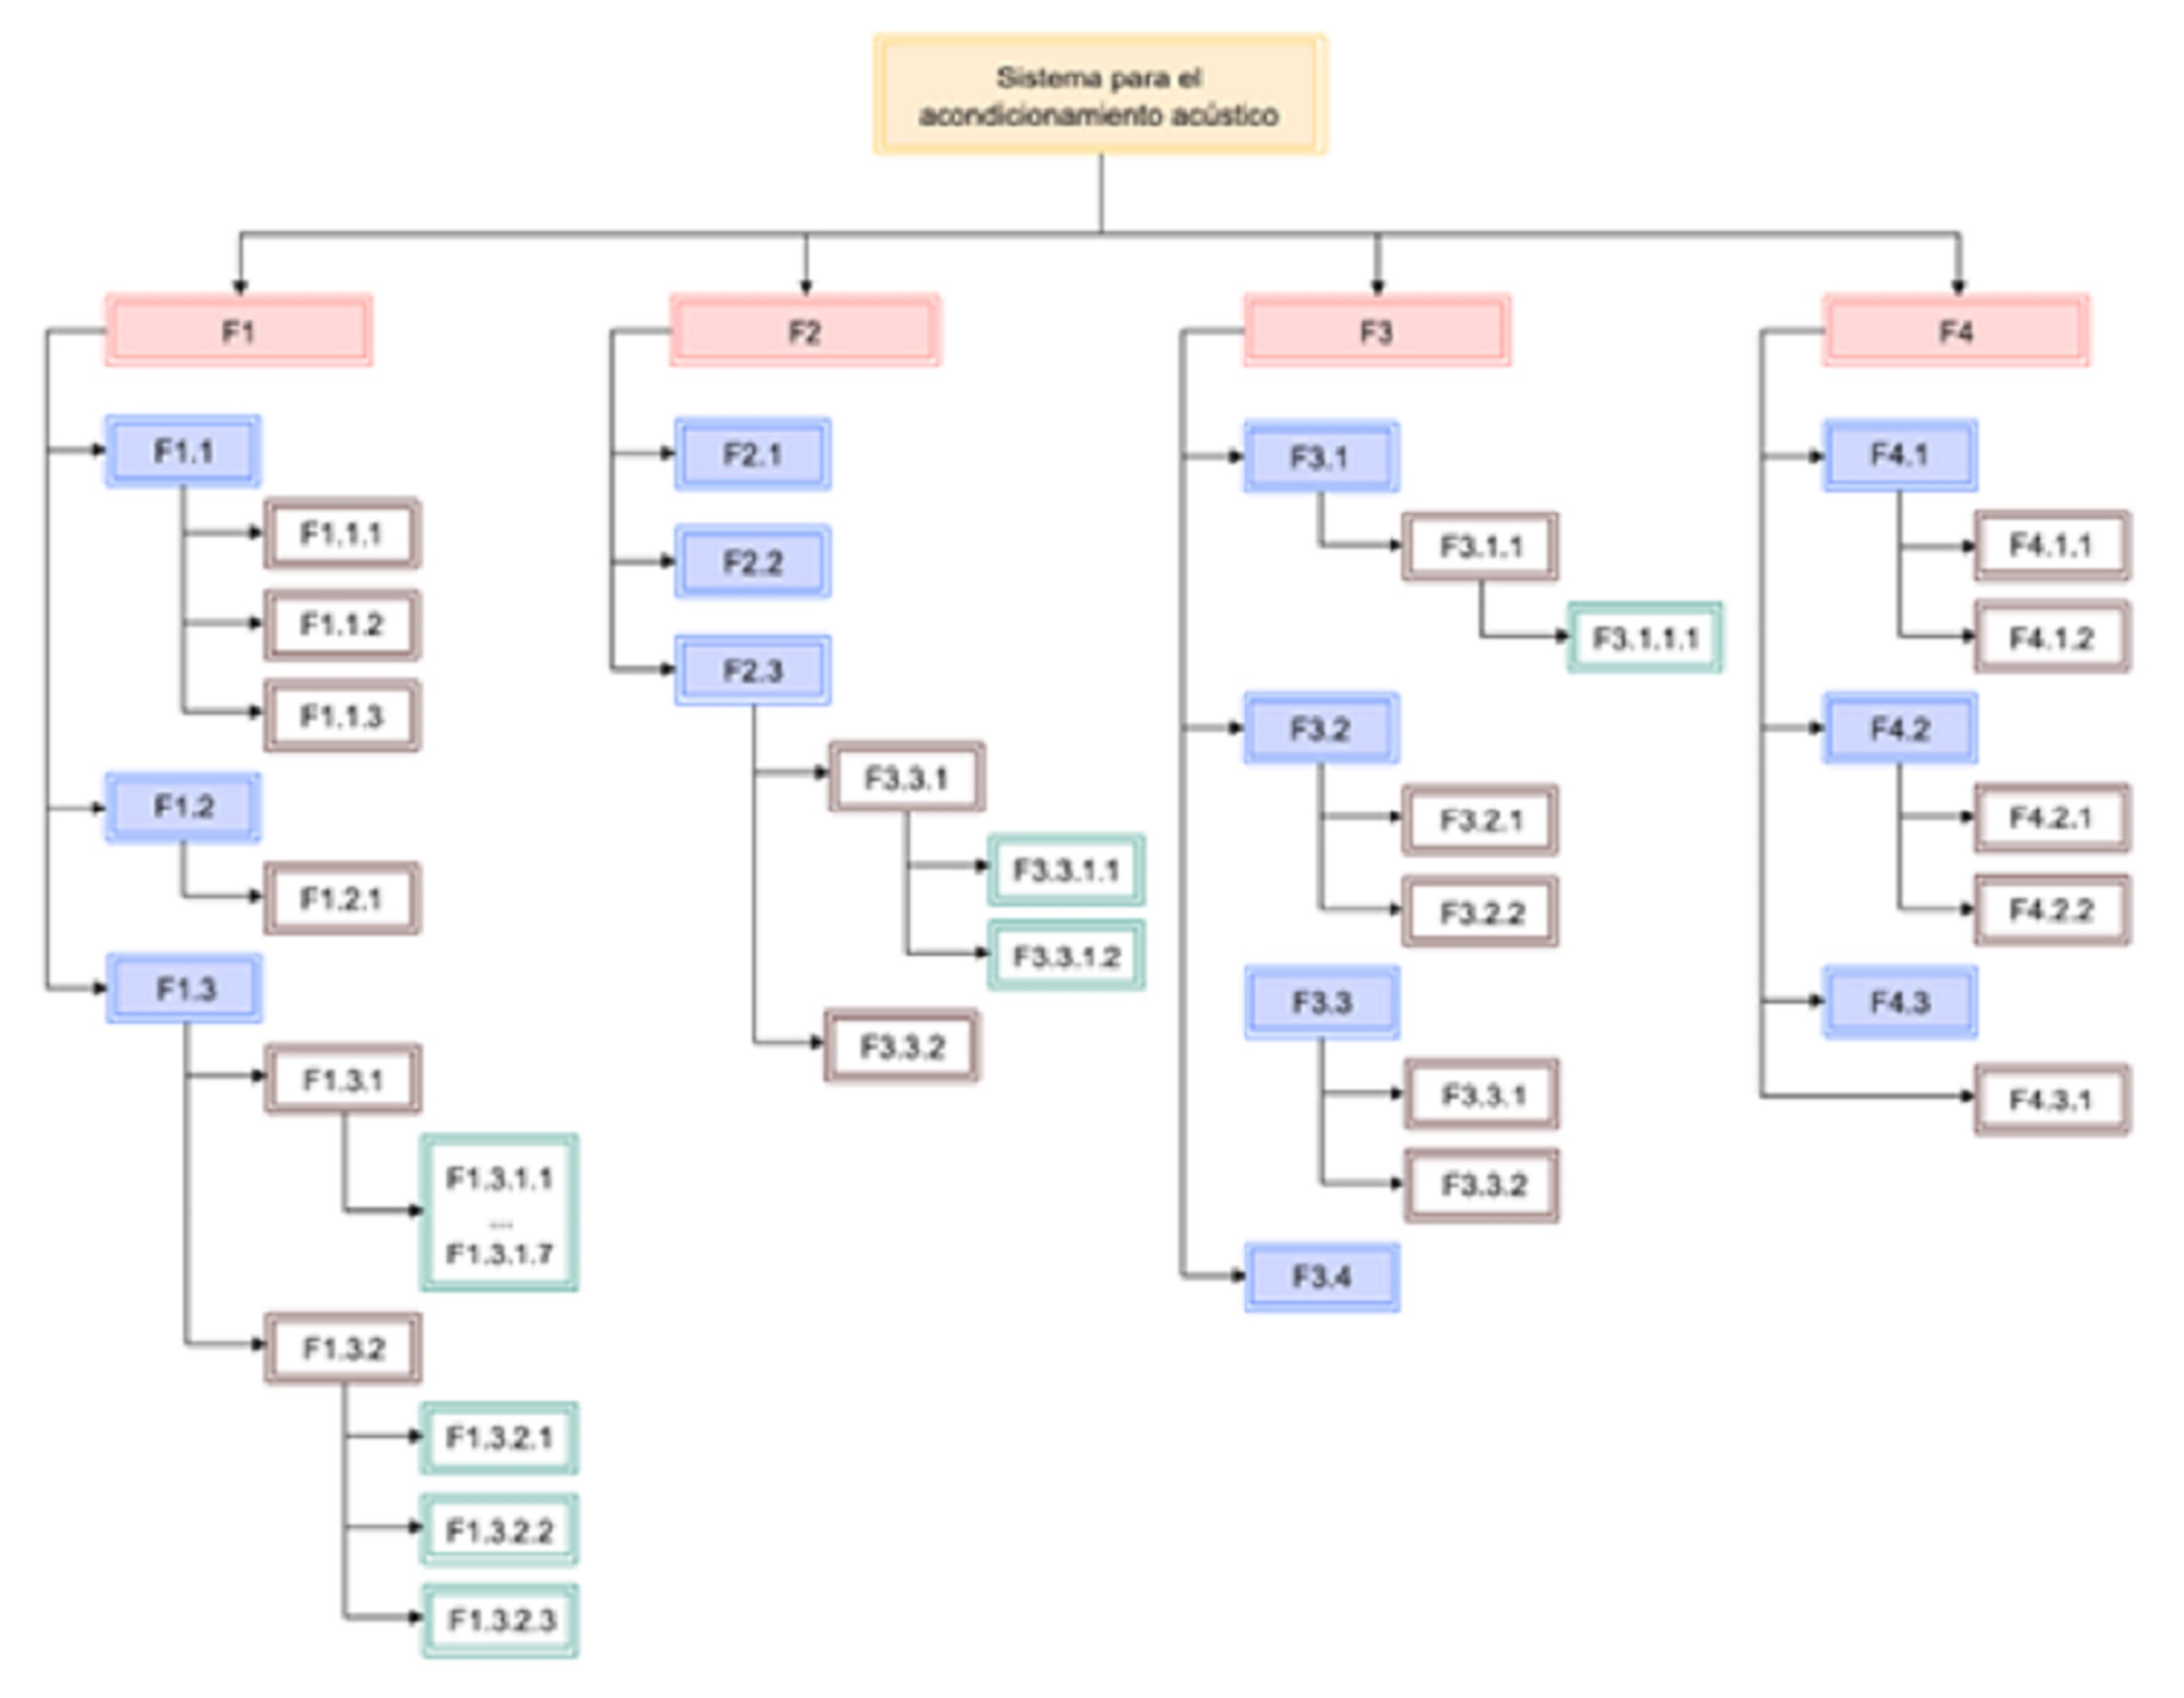
\includegraphics[width=0.8\textwidth]{imagenes/5.jpg}
    \caption{\footnotesize Diagrama de las funciones del sistema para el tratamiento acústico.}
    \label{fig:DiagramaFunciones}
\end{figure}
\FloatBarrier
%---------------------Imagenes de los idefs----------------------------------
\begin{figure}[!htb]
    \centering
    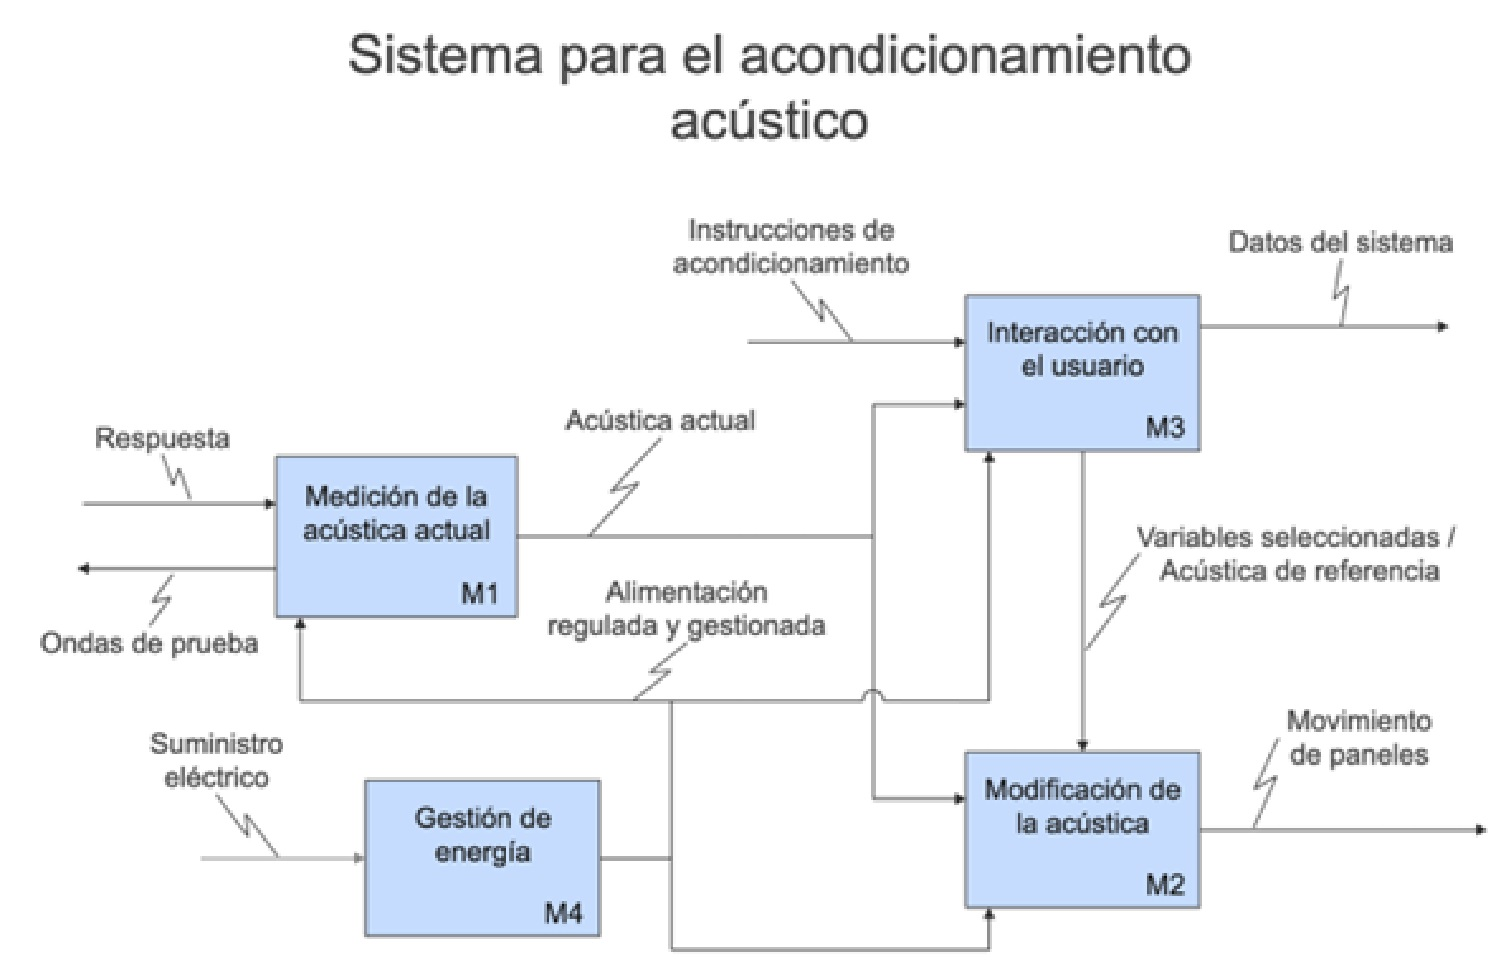
\includegraphics[width=0.8\textwidth]{imagenes/6.jpg}
    \caption{\footnotesize IDEF0 del sistema para el acondicionamiento acústico.}
    \label{fig:IDEF0_Sistema}
\end{figure}
\FloatBarrier

\begin{figure}[!htb]
    \centering
    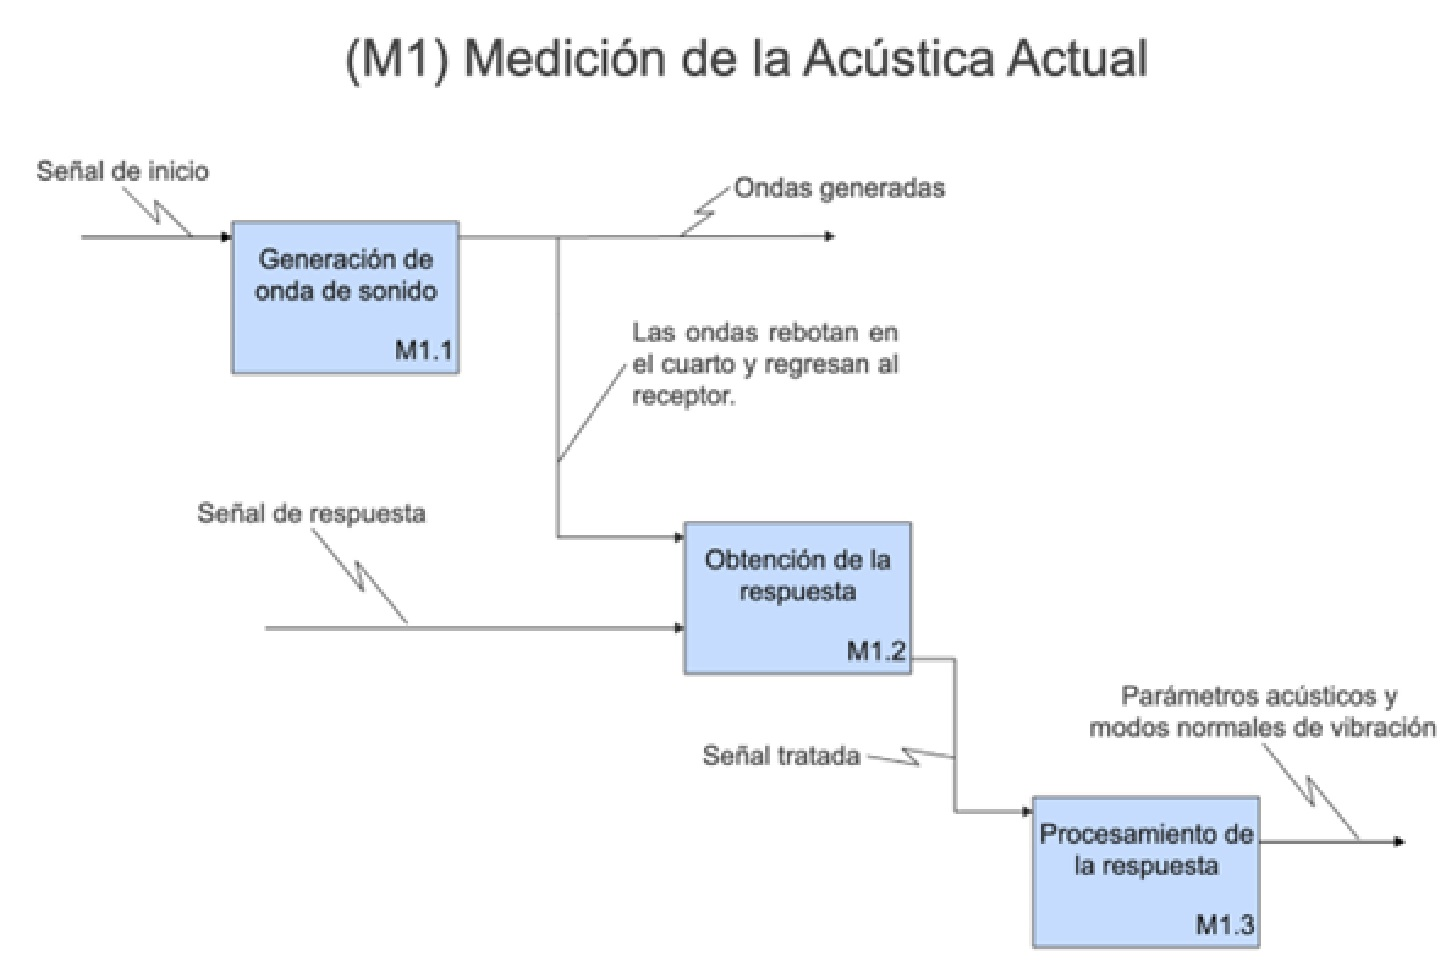
\includegraphics[width=0.8\textwidth]{imagenes/7.jpg}
    \caption{\footnotesize IDEF0 del Módulo de medición de la acústica actual.}
    \label{fig:IDEF0_M1}
\end{figure}
\FloatBarrier

\begin{figure}[!htb]
    \centering
    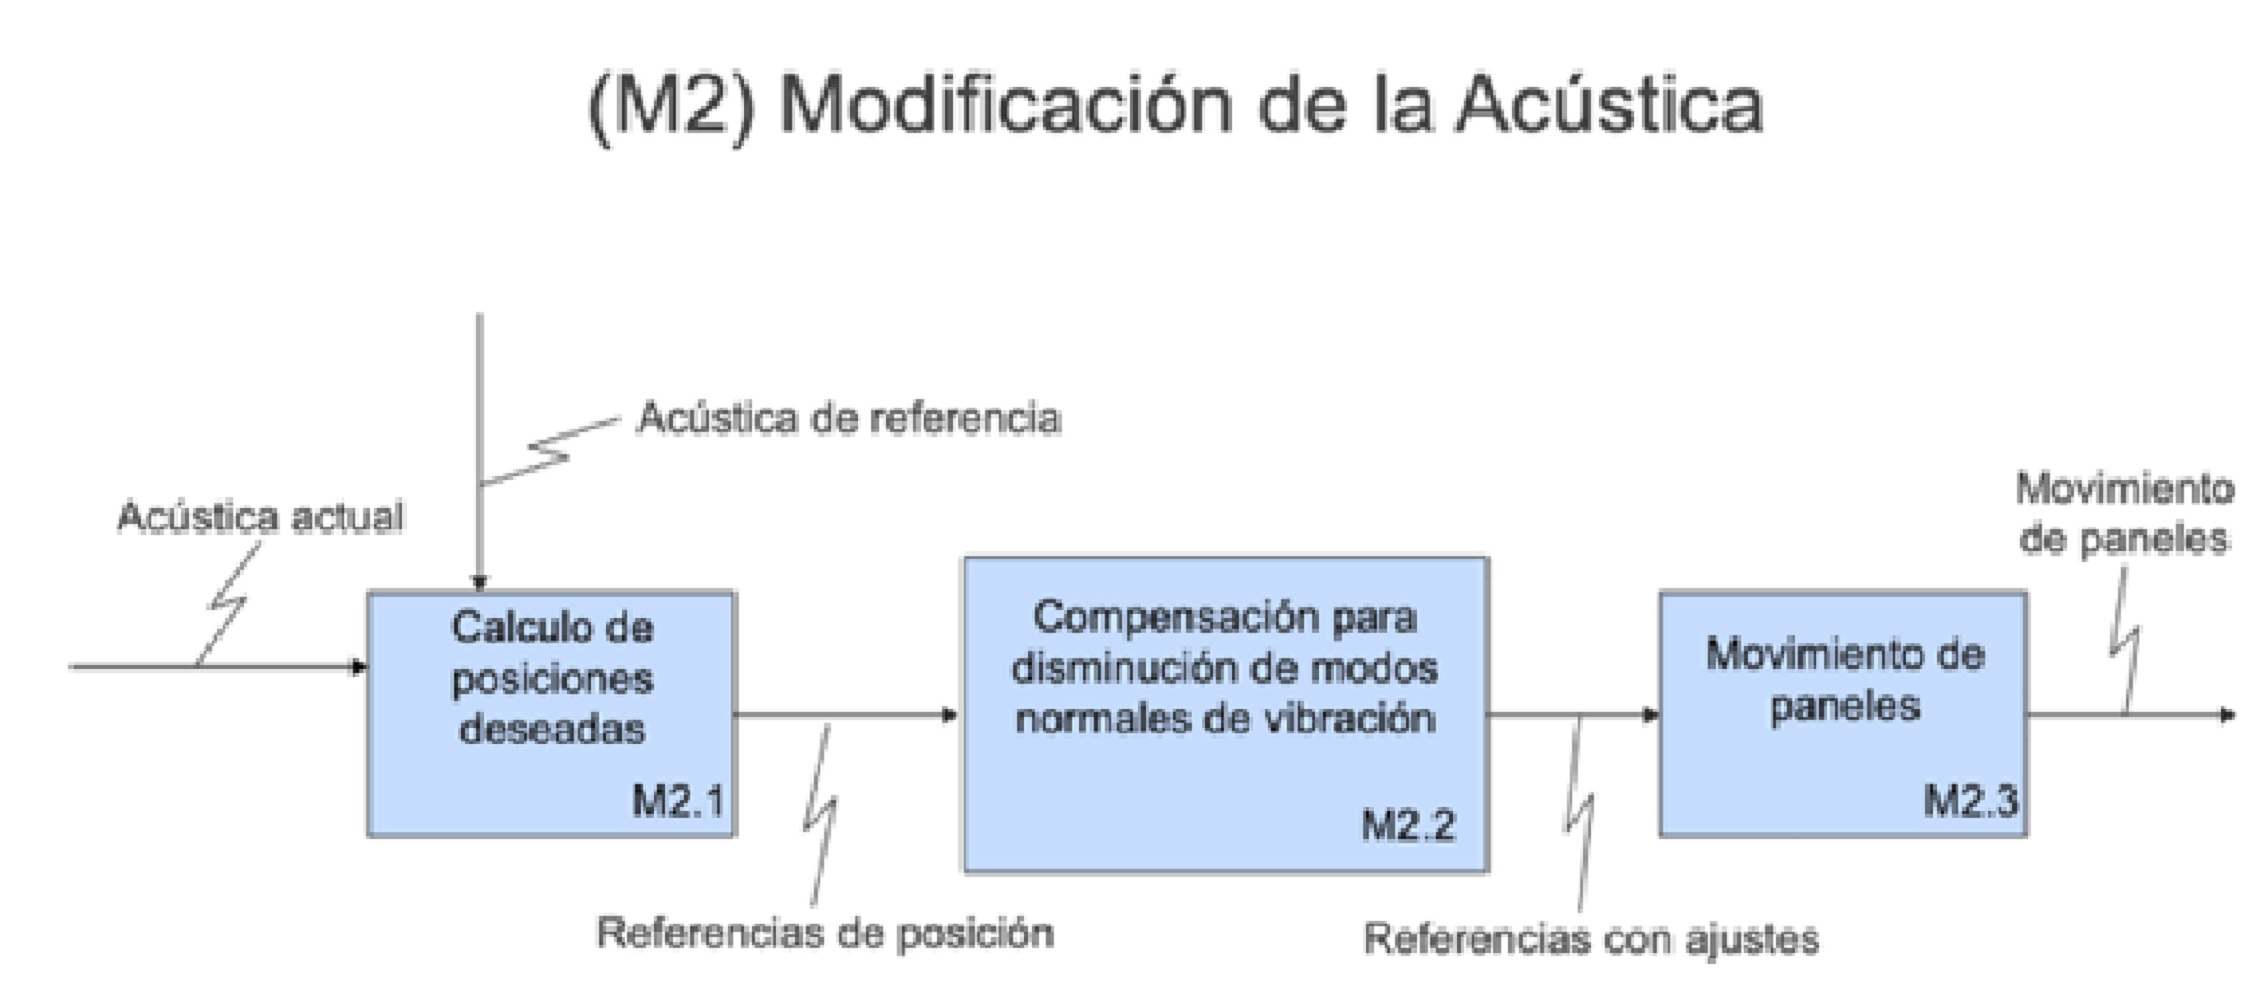
\includegraphics[width=0.8\textwidth]{imagenes/8.jpg}
    \caption{\footnotesize IDEF0 del Módulo de modificación de la acústica.}
    \label{fig:IDEF0_M2}
\end{figure}
\FloatBarrier

\begin{figure}[!htb]
    \centering
    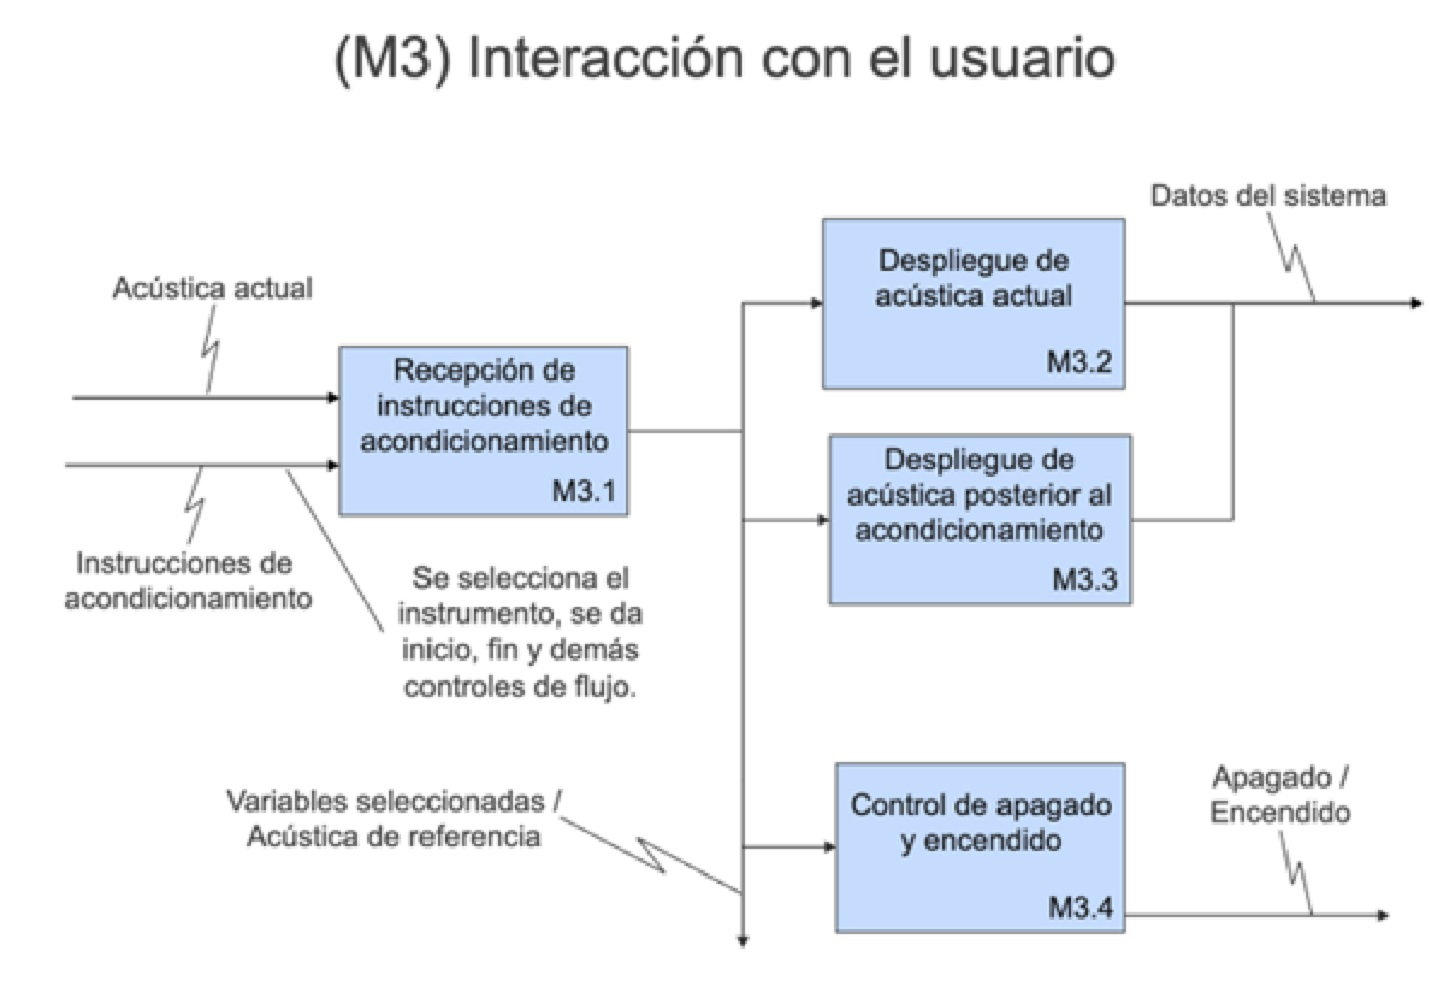
\includegraphics[width=0.8\textwidth]{imagenes/9.jpg}
    \caption{\footnotesize IDEF0 del Módulo de interacción con el usuario.}
    \label{fig:IDEF0_M3}
\end{figure}
\FloatBarrier

\begin{figure}[!htb]
    \centering
    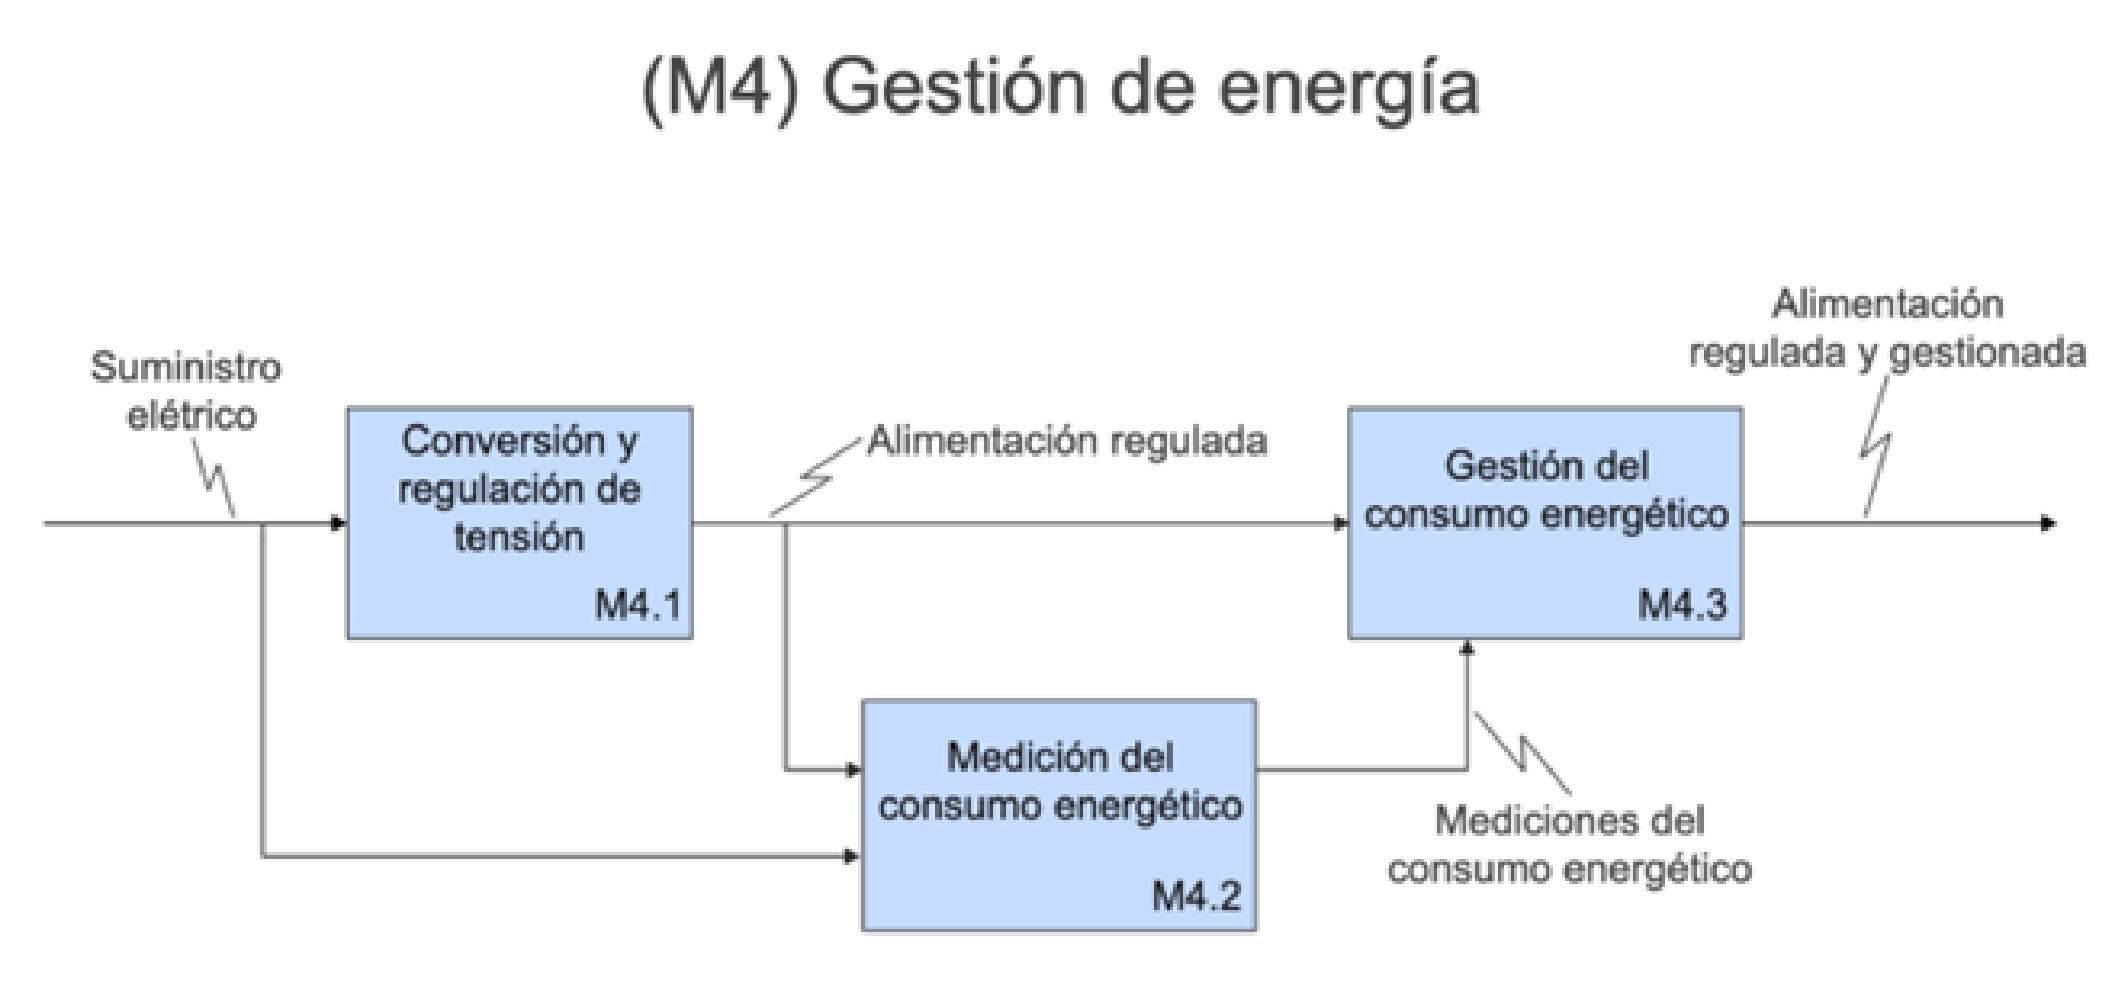
\includegraphics[width=0.8\textwidth]{imagenes/10.jpg}
    \caption{\footnotesize IDEF0 del Módulo de gestión de energía.}
    \label{fig:IDEF0_M4}
\end{figure}
\FloatBarrier
%---------------------Imagenes de los idefs----------------------------------
Se procedió a validar la relación entre los requerimientos y las funciones, para lo cual se elaboró la matriz de trazabilidad presentada en la Tabla “Matriz de trazabilidad requerimientos-funciones”.

%-------------Matriz de trazabilidad requerimientos-funciones--------------------
\definecolor{gr}{gray}{.5}
\begin{center}
\footnotesize
    \begin{longtable}[!htb]{| m{2em} || m{2em} | m{2em}| m{2em}| m{2em}| m{2em}| m{2em}| m{2em}| m{2em}| m{2em}| m{2em}| m{2em}| m{2em}| m{2em}|}
    \hline
    &F1.1 &F1.2 &F1.3 &F2.1 &F2.2 &F2.3 &F3.1 &F3.2 &F3.3 &F3.4 &F4.1 &F4.2 &F4.3\\
    \hline\hline
    R1 & & \cellcolor{gr}{}&\cellcolor{gr}{} &\cellcolor{gr}{} & \cellcolor{gr}{}&\cellcolor{gr}{}&\cellcolor{gr}{} & & & & & & \\
    \hline
    R2 &\cellcolor{gr}{} &\cellcolor{gr}{} & & &\cellcolor{gr}{} & & & & & & & &\\
    \hline
    R3 &\cellcolor{gr}{} & \cellcolor{gr}{}& & &\cellcolor{gr}{} & & & & & & & &\\
    \hline
    R4 &\cellcolor{gr}{} &\cellcolor{gr}{} &\cellcolor{gr}{} & & & & &\cellcolor{gr}{} &\cellcolor{gr}{} & & & &\\
    \hline
    R5 &\cellcolor{gr}{} &\cellcolor{gr}{} &\cellcolor{gr}{} & & & & &\cellcolor{gr}{} &\cellcolor{gr}{} & & & &\\
    \hline
    R6 &\cellcolor{gr}{} &\cellcolor{gr}{} &\cellcolor{gr}{} & & & & &\cellcolor{gr}{} &\cellcolor{gr}{} & & & &\\
    \hline
    R7 &\cellcolor{gr}{} &\cellcolor{gr}{} &\cellcolor{gr}{} & & & & &\cellcolor{gr}{} &\cellcolor{gr}{} & & & &\\
    \hline
    R8 &\cellcolor{gr}{} &\cellcolor{gr}{} &\cellcolor{gr}{} & & & & &\cellcolor{gr}{} &\cellcolor{gr}{} & & & &\\
    \hline
    R9 &\cellcolor{gr}{} &\cellcolor{gr}{} &\cellcolor{gr}{} & & & & &\cellcolor{gr}{} &\cellcolor{gr}{} & & & &\\
    \hline
    R10 &\cellcolor{gr}{} &\cellcolor{gr}{} &\cellcolor{gr}{} & & & & &\cellcolor{gr}{} &\cellcolor{gr}{} & & & &\\
    \hline
    R11 & & & &\cellcolor{gr}{} &\cellcolor{gr}{} & \cellcolor{gr}{}& & & & & & &\\
    \hline
    R12 & & & &\cellcolor{gr}{} &\cellcolor{gr}{} &\cellcolor{gr}{} & & & & & & &\\
    \hline
    R13 &\cellcolor{gr}{} &\cellcolor{gr}{} &\cellcolor{gr}{} & & & & &\cellcolor{gr}{} &\cellcolor{gr}{} & & & &\\
    \hline
    R14 & & & &\cellcolor{gr}{} &\cellcolor{gr}{} &\cellcolor{gr}{} & & & & & & &\\
    \hline
    R15 & & & &\cellcolor{gr}{} &\cellcolor{gr}{} &\cellcolor{gr}{} & & & & & & &\\
    \hline
    R16 & & & & & & & & & & & \cellcolor{gr}{}& \cellcolor{gr}{}&\cellcolor{gr}{}\\
    \hline
    R17 & & & & & & & & & & & \cellcolor{gr}{}& \cellcolor{gr}{}&\cellcolor{gr}{}\\
    \hline
    R18 & & & & & & &\cellcolor{gr}{} & & &\cellcolor{gr}{} & & &\\
    \hline
    R19 & & & &\cellcolor{gr}{} &\cellcolor{gr}{} &\cellcolor{gr}{} & & & & & & &\\
    \hline
    R20 & & & &\cellcolor{gr}{} &\cellcolor{gr}{} &\cellcolor{gr}{} & & & & & & &\\
    \hline
    R21 & & & & & & & &\cellcolor{gr}{} &\cellcolor{gr}{} & & & &\\
    \hline

    \caption{\footnotesize Matriz de trazabilidad requerimientos-funciones.}
    \label{tab:MatTraza_ReqFun}
    \end{longtable}
\end{center}

%-------------Matriz de trazabilidad requerimientos-funciones--------------------
\subsubsection{Arquitectura física}
Para dar forma a la parte física del proyecto se definen los módulos que darán integridad a la propuesta de solución. La arquitectura física del sistema es representada por la transformación de las funciones en módulos, que tomarán parte en los ensambles y componentes físicos. La arquitectura física está planteada para ser capaz de realizar las funciones descritas en la arquitectura funcional y cumplir con los requerimientos del sistema para lograr el funcionamiento deseado.

\begin{enumerate}[{MF}1]
    \item Módulo de procesamiento: Es un módulo cuya función principal es el procesamiento de las ondas de sonido, el cálculo de las posiciones de los paneles y el procesamiento de los comandos ingresados por el usuario. El módulo se define en submódulos, donde el submódulo \textbf{MF}$_{1.1}$ es el encargado de procesar la respuesta del estudio y realizar los cálculos de los parámetros acústicos y los modos normales de vibración. En el submódulo \textbf{MF}$_{1.2}$ se generan los cálculos de las posiciones deseadas de los paneles, así como el procesamiento de la estrategia de control para el movimiento de los mismos, contemplando la medición y el cálculo del error de posición, para que la localización de los paneles sea fiable. El submódulo \textbf{MF}$_{1.3}$ se encarga de procesar todas las instrucciones de acondicionamiento ingresadas por el usuario, así como de todos los parámetros acústicos que se despliegan en la interfaz de muestreo.

    \item Módulo de generación y medición de la acústica: Tiene la función de generar las ondas que excitan el estudio (\textbf{MF}$_{2.1}$) y medir la interacción de las ondas con el recinto (\textbf{MF}$_{2.2}$). El submódulo de la generación de las ondas de sonido funciona a partir de un algoritmo que genera una señal se excitación que es transmitida al estudio mediante una bocina, las ondas que son transmitidas se encargan de describir las características del estudio. Así, las señales que interactúan con el estudio posteriormente son recibidas por el submódulo de medición que consta de un micrófono que capta todas las señales que han interactuado con el recinto.

    \item Módulo modificador de la acústica: Este módulo tiene la función de generar el movimiento de los paneles acústicos considerando la compensación para disminuir los modos normales de vibración (\textbf{MF}$_{3.1}$). El movimiento se lleva a cabo mediante un mecanismo que permite su colocación en un punto donde se requiere modificar la superficie que entra en contacto con las ondas sonoras, este mecanismo es capaz de sensar el error de posición con el propósito de que el lugar en el que el módulo requiere la localización del panel sea específicamente la solicitada. 

    \item Módulo interfaz de usuario: Además de gestionar el encendido y apagado del sistema, el submódulo de interacción directa (\textbf{MF}$_{4.1}$) se encarga de recibir las instrucciones por parte del usuario para el acondicionamiento del estudio, es decir, la selección del instrumento. Al seleccionar el instrumento la consola muestra a través del submódulo de muestreo de datos (\textbf{MF}$_{4.2}$) la acústica ideal para dicho instrumento y posteriormente de que el módulo dos realiza el acondicionamiento se muestran los nuevos valores de las variables acústicas. De igual forma la interfaz muestra las variables acústicas antes de realizar el proceso de acondicionamiento y las frecuencias de vibración que son un problema para el sistema.

    \item Módulo gestor de energía: Se encarga de gestionar el suministro eléctrico requerido por cada uno de los módulos y submódulos. El submódulo de conversión y regulación de la tensión de entrada (\textbf{MF}$_{5.1}$) convierte y regula la señal de corriente alterna que es suministrada al sistema dependiendo de las características de alimentación de cada uno de los componentes del sistema. El módulo es capaz de gestionar el consumo energético del sistema y sus componentes, además de disminuir proporcionalmente la potencia en contra del consumo, lográndolo a través del submódulo de medición del consumo energético (\textbf{MF}$_{5.2}$), es decir, la medición de la tensión de entrada y la corriente que demanda el sistema.
\end{enumerate}

De igual manera se realizó la validación de los módulos y submódulos acorde a las funciones planteadas para el sistema, haciendo uso de la matriz de trazabilidad que se muestra a continuación.


%----------------------Matriz de trazabilidad--------------------------
\definecolor{gr}{gray}{.5}
\begin{center}
\footnotesize
    \begin{longtable}[!htb]{| m{3em} || m{3em} | m{3em}| m{3em}| m{3em}| m{3em}| m{3em}| m{3em}| m{3em}| m{3em}| m{3em}|}
    \hline
    & \multicolumn{3}{c|}{\textbf{MF}$_{1}$} & \multicolumn{2}{|c|}{\textbf{MF}$_{2}$} & \textbf{MF}$_{3}$ & \multicolumn{2}{|c|}{\textbf{MF}$_{4}$} & \multicolumn{2}{|c|}{\textbf{MF}$_{5}$}\\
    \cline{2-11}
    & \textbf{MF}$_{1.1}$ & \textbf{MF}$_{1.2}$ & \textbf{MF}$_{1.3}$ & \textbf{MF}$_{2.1}$ & \textbf{MF}$_{2.2}$ & \textbf{MF}$_{3.1}$ & \textbf{MF}$_{4.1}$ & \textbf{MF}$_{4.2}$ & \textbf{MF}$_{5.1}$ & \textbf{MF}$_{5.2}$ \\
    \hline\hline
    
    \textbf{F}$_{1.1}$ & & & & \cellcolor{gr}{} & & & & & & \\
    \hline
    \textbf{F}$_{1.2}$ & & & & & \cellcolor{gr}{} & & & & & \\
    \hline
    \textbf{F}$_{1.3}$ & \cellcolor{gr}{}& & & & & & & & & \\
    \hline
    \textbf{F}$_{2.1}$ & & \cellcolor{gr}{}& & & & & & & & \\
    \hline
    \textbf{F}$_{2.2}$ & & \cellcolor{gr}{}& & & & \cellcolor{gr}{} & & & & \\
    \hline
    \textbf{F}$_{2.3}$ & & & & & & \cellcolor{gr}{} & & & & \\
    \hline
    \textbf{F}$_{3.1}$ & & & \cellcolor{gr}{} & & & & \cellcolor{gr}{} & & & \\
    \hline
    \textbf{F}$_{3.2}$ & & & \cellcolor{gr}{} & & & & & \cellcolor{gr}{} & & \\
    \hline
    \textbf{F}$_{3.3}$ & & & \cellcolor{gr}{} & & & & & \cellcolor{gr}{} & & \\
    \hline
    \textbf{F}$_{3.4}$ & & & & & & & \cellcolor{gr}{} & & & \\
    \hline
    \textbf{F}$_{4.1}$ & & & & & & & & & \cellcolor{gr}{} & \\
    \hline
    \textbf{F}$_{4.2}$ & & & & & & & & & & \cellcolor{gr}{} \\
    \hline
    \textbf{F}$_{4.3}$ & & & & & & & & & & \cellcolor{gr}{} \\
    \hline
    
    \caption{\footnotesize Matriz de trazabilidad de arquitectura física}
    \label{tab:MatTrazArquiFis}
    \end{longtable}
\end{center}
%----------------------Matriz de trazabilidad--------------------------
\begin{figure}[!htb]
    \centering
    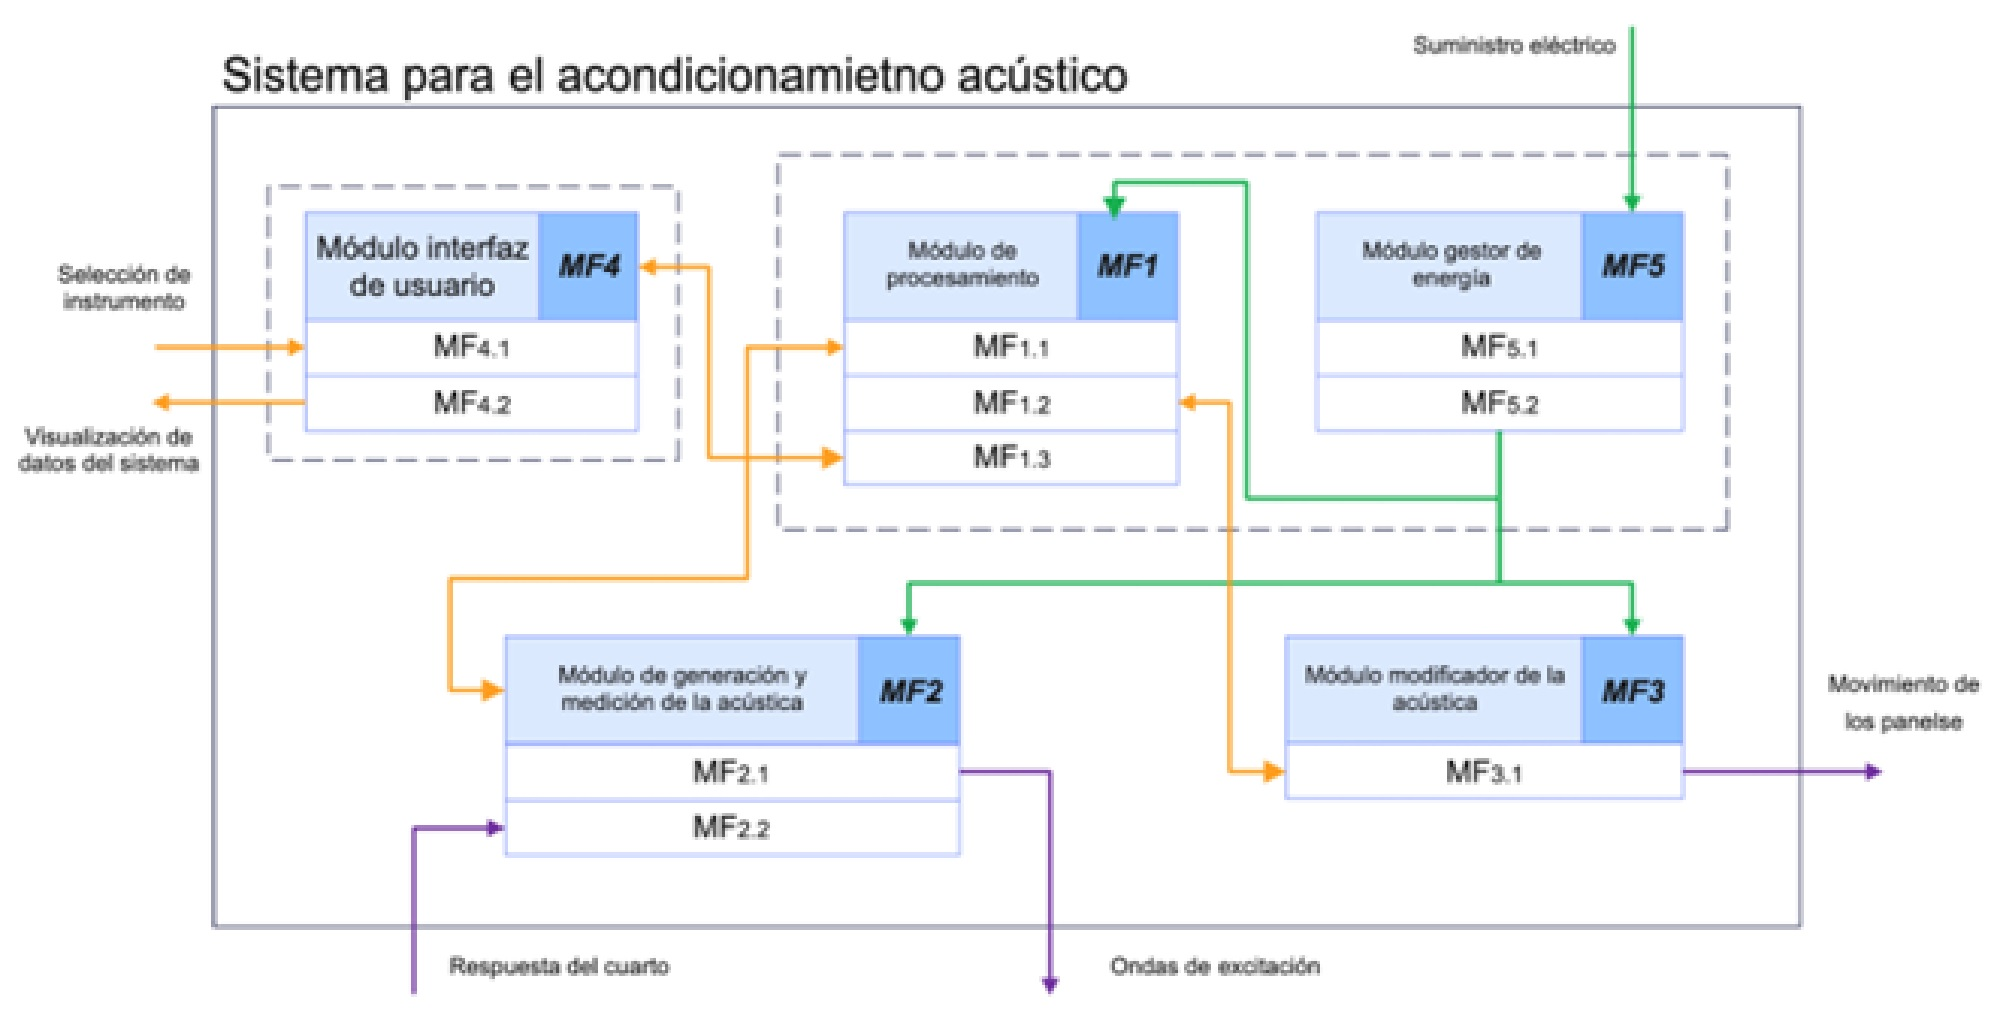
\includegraphics[width=1\textwidth]{imagenes/sistema para acondicionamiento.jpg}
    \caption{\footnotesize Diagrama del sistema para el acondicionamiento acústico}
    \label{fig:DiagramaSistema}
\end{figure}
\FloatBarrier

\subsubsection{Propuesta de solución}
Para desarrollar la propuesta de solución, primero se hizo uso de la matriz morfológica para observar las diferentes alternativas que se tienen para cada uno de los sistemas. La matriz morfológica toma los aspectos mas relevantes del diseño físico y las diferentes soluciones. Lo anterior nos permitirá generar diferentes conceptos solución, que sean combinaciones de las alternativas de solución para los diferentes sistemas.
Es necesario hacer una valoración de los conceptos solución, y para este propósito, es necesario contar con criterios que nos permitan separar los unos de los otros. De acuerdo a la metodología, se hará uso del Proceso Analítico Jerárquico (AHP por sus siglas en ingles).

\begin{itemize}
    \item $C_{r1}$ Velocidad de actuación
    \item $C_{r2}$ Peso
    \item $C_{r3}$ Complejidad del mecanismo
    \item $C_{r4}$ Cantidad de actuadores
    \item $C_{r5}$ Costo de la actuación
    \item $C_{r6}$ Resolución acústica
    \item $C_{r7}$ Repetibilidad
    \item $C_{r8}$ Consumo energético
    \item $C_{r9}$ Variedad de potencias consumidas
    \item $C_{r10}$ Facilidad del control de la actuación
    \item $C_{r11}$ Tamaño
    \item $C_{r12}$ Confiabilidad del sistema de actuación
    \item $C_{r13}$ Complejidad de manufactura del mecanismo de actuación
    \item $C_{r14}$ Error de posición 
    \item $C_{r15}$ Cantidad de hardware externo al equipo de computo personal
    \item $C_{r16}$ Relación entre señal y ruido
    \item $C_{r17}$ Sensibilidad del micrófono
    \item $C_{r18}$ Potencia de procesado de la tarjeta embebida
    \item $C_{r19}$ Potencia de procesado del equipo de computo
    \item $C_{r20}$ Simplicidad de la medición en el error de posición
    \item $C_{r21}$ Robustez necesaria del anclaje
    \item $C_{r22}$ Propensión a fallas estructurales
    \item $C_{r23}$ Propensión a fallas eléctricas
    \item $C_{r24}$ Facilidad para saltar entre disposiciones 
    \item $C_{r25}$ Modularidad
    \item $C_{r26}$ Costo de la electrónica embebida
    \item $C_{r27}$ Cantidad de paneles utilizados
\end{itemize}
La mayoría de los criterios enlistados anteriormente están íntimamente relacionados con la forma en la que el sistema mueve los paneles a lo largo del cuarto, por lo que la generación de conceptos solución, tendrán como eje principal, las diferentes formas de movimiento de los paneles.
Algunas de las alternativas de solución para sistemas específicos, son compatibles con diferentes propuestas de solución, por lo que se estudiaran aparte y se adjuntaran al concepto solución elegido en base a los criterios que si son propios del mismo.
\definecolor{gr_l}{gray}{.8}
%-----------------------------Matriz Morfológica-----------------------------
\begin{center}
\scriptsize
\centering
    \begin{longtable}[!htb]{|>{\centering\arraybackslash}m{3em} ||>{\centering\arraybackslash}m{8em} | >{\centering\arraybackslash}m{8em}| >{\centering\arraybackslash}m{8em}| >{\centering\arraybackslash}m{8em}|>{\centering\arraybackslash}m{8em}|}
    \hline
    & \textbf{Características} & \textbf{Alternativa 1} & \textbf{Alternativa 2}& \textbf{Alternativa 3}& \textbf{Alternativa 4}\\
    \hline\hline
    \textbf{$C_1$} & Forma de movimiento de los paneles & Rotacional en base prismática & Tipo pick and place & Construcción y movimiento de líneas & Paneles en configuración plegable\\
    \hline
    \textbf{$C_2$} & Método para la reflexión & Paneles de reflexión & Pared de fondo & - & -\\
    \hline
    \textbf{$C_3$} & Grabación en varias posiciones & No & Manual & Automático & Con múltiples micrófonos\\
    \hline
    \textbf{$C_4$} & Generación de ondas de sonido & Bocina de equipo de cómputo & Bocina externa & Bocina para circuitos & - \\
    \hline
    \textbf{$C_5$} & Dispositivo de grabación & Micrófono de equipo de cómputo & Micrófono externo & Micrófono para circuitos & - \\
    \hline
    \textbf{$C_6$} & Plataforma de cálculo para las posiciones deseadas & Equipo de cómputo & Microcontrolador embebido & FPGA & - \\
    \hline
    \textbf{$C_7$} & Plataforma de procesado del control & Equipo de cómputo & Microcontrolador embebido & FPGA & - \\
    \hline
    \textbf{$C_8$} & Plataforma para procesado de la acústica & Equipo de cómputo & Microcontrolador embebido & FPGA & - \\
    \hline
    \textbf{$C_9$} & Sensado de las posiciones de los paneles & Encoders & Sensores de contacto & Visión artificial & Sensor de flexión \\
    \hline
    \textbf{$C_{10}$} & Plataforma de visualización de información & Equipo de cómputo & Pantalla OLED & Pantalla LCD & - \\
    \hline
    \textbf{$C_{11}$} & Control de interfaz & Pantalla táctil & Botonera & Ratón y teclado & - \\
    \hline
    \textbf{$C_{12}$} & Encapsulado de sistemas embebidos & Si & No & - & - \\
    \hline
    \textbf{$C_{13}$} & Inclusión del sistema energético en el sistema embebido & Si & No & - & - \\
    \hline
    \textbf{$C_{14}$} & Anclaje al suelo & Si & No & - & - \\
    \hline
    \textbf{$C_{15}$} & Método de anclaje & Tornillos & Colgados & Adhesivos & Magnéticos \\
    \hline
    \textbf{$C_{16}$} & Método de comunicación & Serial & Wi-fi & Bluetooth & - \\
    \hline

    \caption{Matriz morfológica}
    \label{tab:Matriz morfológica}
    \end{longtable}
\end{center}
%-----------------------------Matriz Morfológica-----------------------------

En base a las diferentes alternativas, se crearon 4 conceptos de solución, cuya mayor diferencia es el método de movimiento para los paneles. Debido a que hay alternativas que no son dependientes del método de movimiento, la selección de estas se hará independientemente. 
%-----------------------------Conceptos solución-----------------------------
\begin{center}
\scriptsize
\centering
    \begin{longtable}[!htb]{|>{\centering\arraybackslash}m{3em} ||>{\centering\arraybackslash}m{8em} | >{\centering\arraybackslash}m{8em}| >{\centering\arraybackslash}m{8em}| >{\centering\arraybackslash}m{8em}|>{\centering\arraybackslash}m{8em}|}
    \hline
    & \textbf{Características} & \textbf{$CS_1$} & \textbf{$CS_2$}& \textbf{$CS_3$}& \textbf{$CS_4$}\\
    \hline\hline
    \textbf{$C_1$} & Forma de movimiento de los paneles & Rotacional en base prismática & Tipo pick and place & Construcción y movimiento de líneas & Paneles en configuración plegable\\
    \hline
    \textbf{$C_2$} & Tipo de actuación & Con motor y acopladores magnéticos & Con motor y actuador magnético & Con motores & Motores lineales\\
    \hline
    \textbf{$C_3$} & Sensado de las posiciones de los paneles & Encoders, sensores de contacto o visión artificial & Encoders o visión artificial & Encoders & Sensores de flexión\\
    \hline
    \textbf{$C_4$} & Posicionamiento de paneles & Anclados a la base prismática & Acoplamiento en pared & Acoplado a un cable & Acoplados entre si\\
    \hline
    \textbf{$C_5$} & Sistema de alimentación de paneles & No & Si & Si & No \\
    \hline

    \caption{Conceptos solución}
    \label{tab:ConceptosSolucion}
    \end{longtable}
\end{center}
%-----------------------------Conceptos solución---------------------------------
Primero se hará la comparación de los diferentes conceptos solución con base en cada uno de los criterios. Es importante notar que no todos los criterios se pueden aplicar para discernir entre los diferentes conceptos solución, por tanto, esos criterios se aplicaran a las alternativas que se analizaran individualmente.
%-------------------------CR1 Velocidad de actuación-----------------------------
\begin{table}[!htbp]
    \begin{minipage}[b]{0.5\linewidth}
        \scriptsize
        \centering
            \begin{tabular}{|>{\centering\arraybackslash}m{2em} ||>{\centering\arraybackslash}m{2em} | >{\centering\arraybackslash}m{2em}| >{\centering\arraybackslash}m{2em}| >{\centering\arraybackslash}m{2em}|}
            \hline
            & \textbf{$CS_1$} & \textbf{$CS_2$}& \textbf{$CS_3$}& \textbf{$CS_4$}\\
            \hline\hline
            \textbf{$CS_1$} & \cellcolor{gr_l}{1}  &  10  &    5   &   2    \\
            \textbf{$CS_2$} & 0.10 &  \cellcolor{gr_l}{1} &  0.50  &  0.20  \\
            \textbf{$CS_3$} & 0.20 &  2   &  \cellcolor{gr_l}{1}   &  0.40  \\
            \textbf{$CS_4$} & 0.50 &  5   &  2.50  &   \cellcolor{gr_l}{1}  \\ 
            \hline
        \end{tabular}
        \caption{Matriz de comparación de $Cr_1$}
        \label{tab:MComCr1}
    \end{minipage}
    \begin{minipage}[b]{0.5\linewidth}
        \scriptsize
        \centering
            \begin{tabular}{|>{\centering\arraybackslash}m{2em} ||>{\centering\arraybackslash}m{2em} | >{\centering\arraybackslash}m{2em}| >{\centering\arraybackslash}m{2em}| >{\centering\arraybackslash}m{2em}|>{\centering\arraybackslash}m{2em}|}
            \hline
            & \textbf{$CS_1$} & \textbf{$CS_2$}& \textbf{$CS_3$}& \textbf{$CS_4$}& \textbf{$V_{Cr_1}$}\\
            \hline\hline
            \textbf{$CS_1$} & 0.56 &  0.56  &   0.56   &  0.56  &  0.56   \\
            \textbf{$CS_2$} & 0.06 &  0.06  &   0.06   &  0.06  &  0.06   \\
            \textbf{$CS_3$} & 0.11 &  0.11  &   0.11   &  0.11  &  0.11   \\
            \textbf{$CS_4$} & 0.28 &  0.28  &   0.28   &  0.28  &  0.28   \\ 
            \hline
        \end{tabular}
        \caption{Matriz normalizada de $Cr_1$ y $V_{Cr_1}$}
        \label{tab:MNorm_Cr1}
    \end{minipage}
\end{table}
%-------------------------CR1 Velocidad de actuación-----------------------------

%-------------------------CR2 Peso-----------------------------
\begin{table}[!htbp]
    \begin{minipage}[b]{0.5\linewidth}
        \scriptsize
        \centering
            \begin{tabular}{|>{\centering\arraybackslash}m{2em} ||>{\centering\arraybackslash}m{2em} | >{\centering\arraybackslash}m{2em}| >{\centering\arraybackslash}m{2em}| >{\centering\arraybackslash}m{2em}|}
            \hline
            & \textbf{$CS_1$} & \textbf{$CS_2$}& \textbf{$CS_3$}& \textbf{$CS_4$}\\
            \hline\hline
            \textbf{$CS_1$} & \cellcolor{gr_l}{1} &  0.38  &  0.38   &   1   \\
            \textbf{$CS_2$} & 2.67 &  \cellcolor{gr_l}{1}  &   1     &  2.67  \\
            \textbf{$CS_3$} & 2.67 &  1      &  \cellcolor{gr_l}{1}   &  2.67  \\
            \textbf{$CS_4$} &   1  &  0.38   &  0.38  &   \cellcolor{gr_l}{1}  \\ 
            \hline
        \end{tabular}
        \caption{Matriz de comparación de $Cr_2$}
        \label{tab:MComCr2}
    \end{minipage}
    \begin{minipage}[b]{0.5\linewidth}
        \scriptsize
        \centering
            \begin{tabular}{|>{\centering\arraybackslash}m{2em} ||>{\centering\arraybackslash}m{2em} | >{\centering\arraybackslash}m{2em}| >{\centering\arraybackslash}m{2em}| >{\centering\arraybackslash}m{2em}|>{\centering\arraybackslash}m{2em}|}
            \hline
            & \textbf{$CS_1$} & \textbf{$CS_2$}& \textbf{$CS_3$}& \textbf{$CS_4$}& \textbf{$V_{Cr_2}$}\\
            \hline\hline
            \textbf{$CS_1$} & 0.14 &  0.14  &   0.14   &  0.14  &  0.14   \\
            \textbf{$CS_2$} & 0.36 &  0.36  &   0.36   &  0.36  &  0.36   \\
            \textbf{$CS_3$} & 0.36 &  0.36  &   0.36   &  0.36  &  0.36   \\
            \textbf{$CS_4$} & 0.14 &  0.14  &   0.14   &  0.14  &  0.14   \\ 
            \hline
        \end{tabular}
        \caption{Matriz normalizada de $Cr_2$ y $V_{Cr_2}$}
        \label{tab:MNorm_Cr1}
    \end{minipage}
\end{table}
%-------------------------CR2 Peso-----------------------------

%-------------------------CR3 Complejidad de mecanismo-----------------------------
\begin{table}[!htbp]
    \begin{minipage}[b]{0.5\linewidth}
        \scriptsize
        \centering
            \begin{tabular}{|>{\centering\arraybackslash}m{2em} ||>{\centering\arraybackslash}m{2em} | >{\centering\arraybackslash}m{2em}| >{\centering\arraybackslash}m{2em}| >{\centering\arraybackslash}m{2em}|}
            \hline
            & \textbf{$CS_1$} & \textbf{$CS_2$}& \textbf{$CS_3$}& \textbf{$CS_4$}\\
            \hline\hline
            \textbf{$CS_1$} & \cellcolor{gr_l}{1}  &  2.67  &    4   &   4   \\
            \textbf{$CS_2$} & 0.38 &  \cellcolor{gr_l}{1} &  1.50   &  1.50  \\
            \textbf{$CS_3$} & 0.25 &  0.67   &  \cellcolor{gr_l}{1}   &  1  \\
            \textbf{$CS_4$} & 0.25 &  0.67   &  1  &   \cellcolor{gr_l}{1}  \\ 
            \hline
        \end{tabular}
        \caption{Matriz de comparación de $Cr_3$}
        \label{tab:MComCr3}
    \end{minipage}
    \begin{minipage}[b]{0.5\linewidth}
        \scriptsize
        \centering
            \begin{tabular}{|>{\centering\arraybackslash}m{2em} ||>{\centering\arraybackslash}m{2em} | >{\centering\arraybackslash}m{2em}| >{\centering\arraybackslash}m{2em}| >{\centering\arraybackslash}m{2em}|>{\centering\arraybackslash}m{2em}|}
            \hline
            & \textbf{$CS_1$} & \textbf{$CS_2$}& \textbf{$CS_3$}& \textbf{$CS_4$}& \textbf{$V_{Cr_3}$}\\
            \hline\hline
            \textbf{$CS_1$} & 0.53 &  0.53  &   0.53   &  0.53  &  0.53   \\
            \textbf{$CS_2$} & 0.20 &  0.20  &   0.20   &  0.20  &  0.20   \\
            \textbf{$CS_3$} & 0.13 &  0.13  &   0.13   &  0.13  &  0.13   \\
            \textbf{$CS_4$} & 0.13 &  0.13  &   0.13   &  0.13  &  0.13   \\ 
            \hline
        \end{tabular}
        \caption{Matriz normalizada de $Cr_3$ y $V_{Cr_3}$}
        \label{tab:MNorm_Cr3}
    \end{minipage}
\end{table}
%-------------------------CR3 Complejidad de mecanismo-----------------------------

%-------------------------CR4 Cantidad de actuadores-----------------------------
\begin{table}[!htbp]
    \begin{minipage}[b]{0.5\linewidth}
        \scriptsize
        \centering
            \begin{tabular}{|>{\centering\arraybackslash}m{2em} ||>{\centering\arraybackslash}m{2em} | >{\centering\arraybackslash}m{2em}| >{\centering\arraybackslash}m{2em}| >{\centering\arraybackslash}m{2em}|}
            \hline
            & \textbf{$CS_1$} & \textbf{$CS_2$}& \textbf{$CS_3$}& \textbf{$CS_4$}\\
            \hline\hline
            \textbf{$CS_1$} & \cellcolor{gr_l}{1}  &  1.17  &    1.40   &   3.50   \\
            \textbf{$CS_2$} & 0.86 &  \cellcolor{gr_l}{1} &  1.20   &  3.00  \\
            \textbf{$CS_3$} & 0.71 &  0.83   &  \cellcolor{gr_l}{1}   &  2.50  \\
            \textbf{$CS_4$} & 0.29 &  0.33   &  0.40  &   \cellcolor{gr_l}{1}  \\ 
            \hline
        \end{tabular}
        \caption{Matriz de comparación de $Cr_4$}
        \label{tab:MComCr4}
    \end{minipage}
    \begin{minipage}[b]{0.5\linewidth}
        \scriptsize
        \centering
            \begin{tabular}{|>{\centering\arraybackslash}m{2em} ||>{\centering\arraybackslash}m{2em} | >{\centering\arraybackslash}m{2em}| >{\centering\arraybackslash}m{2em}| >{\centering\arraybackslash}m{2em}|>{\centering\arraybackslash}m{2em}|}
            \hline
            & \textbf{$CS_1$} & \textbf{$CS_2$}& \textbf{$CS_3$}& \textbf{$CS_4$}& \textbf{$V_{Cr_4}$}\\
            \hline\hline
            \textbf{$CS_1$} & 0.35 &  0.35  &   0.35   &  0.35  &  0.35   \\
            \textbf{$CS_2$} & 0.30 &  0.30  &   0.30   &  0.30  &  0.30   \\
            \textbf{$CS_3$} & 0.25 &  0.25  &   0.25   &  0.25  &  0.25   \\
            \textbf{$CS_4$} & 0.10 &  0.10  &   0.10   &  0.10  &  0.10   \\ 
            \hline
        \end{tabular}
        \caption{Matriz normalizada de $Cr_4$ y $V_{Cr_4}$}
        \label{tab:MNorm_Cr4}
    \end{minipage}
\end{table}
%-------------------------CR4 Cantidad de actuadores-----------------------------

%-------------------------CR5 Costo de la actuación-----------------------------
\begin{table}[!htbp]
    \begin{minipage}[b]{0.5\linewidth}
        \scriptsize
        \centering
            \begin{tabular}{|>{\centering\arraybackslash}m{2em} ||>{\centering\arraybackslash}m{2em} | >{\centering\arraybackslash}m{2em}| >{\centering\arraybackslash}m{2em}| >{\centering\arraybackslash}m{2em}|}
            \hline
            & \textbf{$CS_1$} & \textbf{$CS_2$}& \textbf{$CS_3$}& \textbf{$CS_4$}\\
            \hline\hline
            \textbf{$CS_1$} & \cellcolor{gr_l}{1}  &  0.89  &    1.14   &   4   \\
            \textbf{$CS_2$} & 1.13 &  \cellcolor{gr_l}{1} &  1.29   &  4.50  \\
            \textbf{$CS_3$} & 0.88 &  0.78   &  \cellcolor{gr_l}{1}   &  3.50  \\
            \textbf{$CS_4$} & 0.25 &  0.22   &  0.29  &   \cellcolor{gr_l}{1}  \\ 
            \hline
        \end{tabular}
        \caption{Matriz de comparación de $Cr_5$}
        \label{tab:MComCr5}
    \end{minipage}
    \begin{minipage}[b]{0.5\linewidth}
        \scriptsize
        \centering
            \begin{tabular}{|>{\centering\arraybackslash}m{2em} ||>{\centering\arraybackslash}m{2em} | >{\centering\arraybackslash}m{2em}| >{\centering\arraybackslash}m{2em}| >{\centering\arraybackslash}m{2em}|>{\centering\arraybackslash}m{2em}|}
            \hline
            & \textbf{$CS_1$} & \textbf{$CS_2$}& \textbf{$CS_3$}& \textbf{$CS_4$}& \textbf{$V_{Cr_5}$}\\
            \hline\hline
            \textbf{$CS_1$} & 0.31 &  0.31  &   0.31   &  0.31  &  0.31   \\
            \textbf{$CS_2$} & 0.35 &  0.35  &   0.35   &  0.35  &  0.35   \\
            \textbf{$CS_3$} & 0.27 &  0.27  &   0.27   &  0.27  &  0.27   \\
            \textbf{$CS_4$} & 0.08 &  0.08  &   0.08   &  0.08  &  0.08   \\ 
            \hline
        \end{tabular}
        \caption{Matriz normalizada de $Cr_5$ y $V_{Cr_5}$}
        \label{tab:MNorm_Cr5}
    \end{minipage}
\end{table}
%-------------------------CR5 Costo de la actuación-----------------------------

%-------------------------CR6 Resolución acústica-----------------------------
\begin{table}[!htbp]
    \begin{minipage}[b]{0.5\linewidth}
        \scriptsize
        \centering
            \begin{tabular}{|>{\centering\arraybackslash}m{2em} ||>{\centering\arraybackslash}m{2em} | >{\centering\arraybackslash}m{2em}| >{\centering\arraybackslash}m{2em}| >{\centering\arraybackslash}m{2em}|}
            \hline
            & \textbf{$CS_1$} & \textbf{$CS_2$}& \textbf{$CS_3$}& \textbf{$CS_4$}\\
            \hline\hline
            \textbf{$CS_1$} & \cellcolor{gr_l}{1}  &  0.90  &    0.90   &   2.25   \\
            \textbf{$CS_2$} & 1.11 &  \cellcolor{gr_l}{1} &  1   &  2.50  \\
            \textbf{$CS_3$} & 1.11 &  1   &  \cellcolor{gr_l}{1}   &  2.50  \\
            \textbf{$CS_4$} & 0.44 &  0.40   &  0.40  &   \cellcolor{gr_l}{1}  \\ 
            \hline
        \end{tabular}
        \caption{Matriz de comparación de $Cr_6$}
        \label{tab:MComCr6}
    \end{minipage}
    \begin{minipage}[b]{0.5\linewidth}
        \scriptsize
        \centering
            \begin{tabular}{|>{\centering\arraybackslash}m{2em} ||>{\centering\arraybackslash}m{2em} | >{\centering\arraybackslash}m{2em}| >{\centering\arraybackslash}m{2em}| >{\centering\arraybackslash}m{2em}|>{\centering\arraybackslash}m{2em}|}
            \hline
            & \textbf{$CS_1$} & \textbf{$CS_2$}& \textbf{$CS_3$}& \textbf{$CS_4$}& \textbf{$V_{Cr_6}$}\\
            \hline\hline
            \textbf{$CS_1$} & 0.27 &  0.27  &   0.27   &  0.27  &  0.27   \\
            \textbf{$CS_2$} & 0.30 &  0.30  &   0.30   &  0.30  &  0.30   \\
            \textbf{$CS_3$} & 0.30 &  0.30  &   0.30   &  0.30  &  0.30    \\
            \textbf{$CS_4$} & 0.12 &  0.12  &   0.12   &  0.12  &  0.12   \\ 
            \hline
        \end{tabular}
        \caption{Matriz normalizada de $Cr_6$ y $V_{Cr_6}$}
        \label{tab:MNorm_Cr6}
    \end{minipage}
\end{table}
%-------------------------CR6 Resolución acústica-----------------------------

%-------------------------CR7 Repetibilidad-----------------------------
\begin{table}[!htbp]
    \begin{minipage}[b]{0.5\linewidth}
        \scriptsize
        \centering
            \begin{tabular}{|>{\centering\arraybackslash}m{2em} ||>{\centering\arraybackslash}m{2em} | >{\centering\arraybackslash}m{2em}| >{\centering\arraybackslash}m{2em}| >{\centering\arraybackslash}m{2em}|}
            \hline
            & \textbf{$CS_1$} & \textbf{$CS_2$}& \textbf{$CS_3$}& \textbf{$CS_4$}\\
            \hline\hline
            \textbf{$CS_1$} & \cellcolor{gr_l}{1}  &  5  &    3.33   &   1.43   \\
            \textbf{$CS_2$} & 0.20 &  \cellcolor{gr_l}{1} &  0.67   &  0.29  \\
            \textbf{$CS_3$} & 0.30 &  1.50   &  \cellcolor{gr_l}{1}   &  0.43  \\
            \textbf{$CS_4$} & 0.70 &  3.50   &  2.33  &   \cellcolor{gr_l}{1}  \\ 
            \hline
        \end{tabular}
        \caption{Matriz de comparación de $Cr_7$}
        \label{tab:MComCr7}
    \end{minipage}
    \begin{minipage}[b]{0.5\linewidth}
        \scriptsize
        \centering
            \begin{tabular}{|>{\centering\arraybackslash}m{2em} ||>{\centering\arraybackslash}m{2em} | >{\centering\arraybackslash}m{2em}| >{\centering\arraybackslash}m{2em}| >{\centering\arraybackslash}m{2em}|>{\centering\arraybackslash}m{2em}|}
            \hline
            & \textbf{$CS_1$} & \textbf{$CS_2$}& \textbf{$CS_3$}& \textbf{$CS_4$}& \textbf{$V_{Cr_7}$}\\
            \hline\hline
            \textbf{$CS_1$} & 0.45 &  0.45  &   0.45   &  0.45  &  0.45   \\
            \textbf{$CS_2$} & 0.09 &  0.09  &   0.09   &  0.09  &  0.09   \\
            \textbf{$CS_3$} & 0.14 &  0.14  &   0.14   &  0.14  &  0.14    \\
            \textbf{$CS_4$} & 0.32 &  0.32  &   0.32   &  0.32  &  0.32   \\ 
            \hline
        \end{tabular}
        \caption{Matriz normalizada de $Cr_7$ y $V_{Cr_7}$}
        \label{tab:MNorm_Cr7}
    \end{minipage}
\end{table}
%-------------------------CR7 Repetibilidad-----------------------------

%-------------------------CR8 Consumo energético-----------------------------
\begin{table}[!htbp]
    \begin{minipage}[b]{0.5\linewidth}
        \scriptsize
        \centering
            \begin{tabular}{|>{\centering\arraybackslash}m{2em} ||>{\centering\arraybackslash}m{2em} | >{\centering\arraybackslash}m{2em}| >{\centering\arraybackslash}m{2em}| >{\centering\arraybackslash}m{2em}|}
            \hline
            & \textbf{$CS_1$} & \textbf{$CS_2$}& \textbf{$CS_3$}& \textbf{$CS_4$}\\
            \hline\hline
            \textbf{$CS_1$} & \cellcolor{gr_l}{1}  &  3  &    2.25   &   4.50   \\
            \textbf{$CS_2$} & 0.33 &  \cellcolor{gr_l}{1} &   0.75   &  1.50  \\
            \textbf{$CS_3$} & 0.44 &  1.33   &  \cellcolor{gr_l}{1}   &  2  \\
            \textbf{$CS_4$} & 0.22 &  0.67   &  0.50  &   \cellcolor{gr_l}{1}  \\ 
            \hline
        \end{tabular}
        \caption{Matriz de comparación de $Cr_8$}
        \label{tab:MComCr8}
    \end{minipage}
    \begin{minipage}[b]{0.5\linewidth}
        \scriptsize
        \centering
            \begin{tabular}{|>{\centering\arraybackslash}m{2em} ||>{\centering\arraybackslash}m{2em} | >{\centering\arraybackslash}m{2em}| >{\centering\arraybackslash}m{2em}| >{\centering\arraybackslash}m{2em}|>{\centering\arraybackslash}m{2em}|}
            \hline
            & \textbf{$CS_1$} & \textbf{$CS_2$}& \textbf{$CS_3$}& \textbf{$CS_4$}& \textbf{$V_{Cr_8}$}\\
            \hline\hline
            \textbf{$CS_1$} & 0.50 &  0.50  &   0.50   &  0.50  &  0.50   \\
            \textbf{$CS_2$} & 0.17 &  0.17  &   0.17   &  0.17  &  0.17   \\
            \textbf{$CS_3$} & 0.22 &  0.22  &   0.22   &  0.22  &  0.22    \\
            \textbf{$CS_4$} & 0.11 &  0.11  &   0.11   &  0.11  &  0.11   \\ 
            \hline
        \end{tabular}
        \caption{Matriz normalizada de $Cr_8$ y $V_{Cr_8}$}
        \label{tab:MNorm_Cr8}
    \end{minipage}
\end{table}
%-------------------------CR8 Consumo energético-----------------------------

%-------------------------CR9 Variedad de potencias consumidas-----------------------------
\begin{table}[!htbp]
    \begin{minipage}[b]{0.5\linewidth}
        \scriptsize
        \centering
            \begin{tabular}{|>{\centering\arraybackslash}m{2em} ||>{\centering\arraybackslash}m{2em} | >{\centering\arraybackslash}m{2em}| >{\centering\arraybackslash}m{2em}| >{\centering\arraybackslash}m{2em}|}
            \hline
            & \textbf{$CS_1$} & \textbf{$CS_2$}& \textbf{$CS_3$}& \textbf{$CS_4$}\\
            \hline\hline
            \textbf{$CS_1$} & \cellcolor{gr_l}{1}  &  1  &    0.88   &   0.70   \\
            \textbf{$CS_2$} & 1 &  \cellcolor{gr_l}{1} &      0.88   &      0.70  \\
            \textbf{$CS_3$} & 1.14 &  1.14   &  \cellcolor{gr_l}{1}   &  0.80  \\
            \textbf{$CS_4$} & 1.43 &  1.43   &  1.25  &   \cellcolor{gr_l}{1}  \\ 
            \hline
        \end{tabular}
        \caption{Matriz de comparación de $Cr_9$}
        \label{tab:MComCr9}
    \end{minipage}
    \begin{minipage}[b]{0.5\linewidth}
        \scriptsize
        \centering
            \begin{tabular}{|>{\centering\arraybackslash}m{2em} ||>{\centering\arraybackslash}m{2em} | >{\centering\arraybackslash}m{2em}| >{\centering\arraybackslash}m{2em}| >{\centering\arraybackslash}m{2em}|>{\centering\arraybackslash}m{2em}|}
            \hline
            & \textbf{$CS_1$} & \textbf{$CS_2$}& \textbf{$CS_3$}& \textbf{$CS_4$}& \textbf{$V_{Cr_9}$}\\
            \hline\hline
            \textbf{$CS_1$} & 0.22 &  0.22  &   0.22   &  0.22  &  0.22   \\
            \textbf{$CS_2$} & 0.22 &  0.22  &   0.22   &  0.22  &  0.22  \\
            \textbf{$CS_3$} & 0.25 &  0.25  &   0.25   &  0.25  &  0.25    \\
            \textbf{$CS_4$} & 0.31 &  0.31  &   0.31   &  0.31  &  0.31   \\ 
            \hline
        \end{tabular}
        \caption{Matriz normalizada de $Cr_9$ y $V_{Cr_9}$}
        \label{tab:MNorm_Cr9}
    \end{minipage}
\end{table}
%-------------------------CR9 Variedad de potencias consumidas-----------------------------

%----------------------CR10 Facilidad en el control de la actuación--------------------------
\begin{table}[!htbp]
    \begin{minipage}[b]{0.5\linewidth}
        \scriptsize
        \centering
            \begin{tabular}{|>{\centering\arraybackslash}m{2em} ||>{\centering\arraybackslash}m{2em} | >{\centering\arraybackslash}m{2em}| >{\centering\arraybackslash}m{2em}| >{\centering\arraybackslash}m{2em}|}
            \hline
            & \textbf{$CS_1$} & \textbf{$CS_2$}& \textbf{$CS_3$}& \textbf{$CS_4$}\\
            \hline\hline
            \textbf{$CS_1$} & \cellcolor{gr_l}{1}  &  9  &    4.50   &   1.29   \\
            \textbf{$CS_2$} & 0.11 &  \cellcolor{gr_l}{1} &   0.50   &   0.14  \\
            \textbf{$CS_3$} & 0.22 &  2   &  \cellcolor{gr_l}{1}   &  0.29  \\
            \textbf{$CS_4$} & 0.78 &  7   &  3.50  &   \cellcolor{gr_l}{1}  \\ 
            \hline
        \end{tabular}
        \caption{Matriz de comparación de $Cr_{10}$}
        \label{tab:MComCr10}
    \end{minipage}
    \begin{minipage}[b]{0.5\linewidth}
        \scriptsize
        \centering
            \begin{tabular}{|>{\centering\arraybackslash}m{2em} ||>{\centering\arraybackslash}m{2em} | >{\centering\arraybackslash}m{2em}| >{\centering\arraybackslash}m{2em}| >{\centering\arraybackslash}m{2em}|>{\centering\arraybackslash}m{2em}|}
            \hline
            & \textbf{$CS_1$} & \textbf{$CS_2$}& \textbf{$CS_3$}& \textbf{$CS_4$}& \textbf{$V_{Cr_{10}}$}\\
            \hline\hline
            \textbf{$CS_1$} & 0.47 &  0.47  &   0.47   &  0.47  &  0.47   \\
            \textbf{$CS_2$} & 0.05 &  0.05  &   0.05   &  0.05  &  0.05  \\
            \textbf{$CS_3$} & 0.11 &  0.11  &   0.11   &  0.11  &  0.11    \\
            \textbf{$CS_4$} & 0.37 &  0.37  &   0.37   &  0.37  &  0.37   \\ 
            \hline
        \end{tabular}
        \caption{Matriz normalizada de $Cr_{10}$ y $V_{Cr_{10}}$}
        \label{tab:MNorm_Cr10}
    \end{minipage}
\end{table}
%----------------------CR10 Facilidad en el control de la actuación--------------------------

%----------------------CR11 Tamaño--------------------------
\begin{table}[!htbp]
    \begin{minipage}[b]{0.5\linewidth}
        \scriptsize
        \centering
            \begin{tabular}{|>{\centering\arraybackslash}m{2em} ||>{\centering\arraybackslash}m{2em} | >{\centering\arraybackslash}m{2em}| >{\centering\arraybackslash}m{2em}| >{\centering\arraybackslash}m{2em}|}
            \hline
            & \textbf{$CS_1$} & \textbf{$CS_2$}& \textbf{$CS_3$}& \textbf{$CS_4$}\\
            \hline\hline
            \textbf{$CS_1$} & \cellcolor{gr_l}{1}  &  1.60  &    2   &   0.89   \\
            \textbf{$CS_2$} & 0.63 &  \cellcolor{gr_l}{1} &   1.25   &   0.56  \\
            \textbf{$CS_3$} & 0.50 &  0.80   &  \cellcolor{gr_l}{1}   &  0.44  \\
            \textbf{$CS_4$} & 1.13 &  1.80   &  2.25  &   \cellcolor{gr_l}{1}  \\ 
            \hline
        \end{tabular}
        \caption{Matriz de comparación de $Cr_{11}$}
        \label{tab:MComCr11}
    \end{minipage}
    \begin{minipage}[b]{0.5\linewidth}
        \scriptsize
        \centering
            \begin{tabular}{|>{\centering\arraybackslash}m{2em} ||>{\centering\arraybackslash}m{2em} | >{\centering\arraybackslash}m{2em}| >{\centering\arraybackslash}m{2em}| >{\centering\arraybackslash}m{2em}|>{\centering\arraybackslash}m{2em}|}
            \hline
            & \textbf{$CS_1$} & \textbf{$CS_2$}& \textbf{$CS_3$}& \textbf{$CS_4$}& \textbf{$V_{Cr_{11}}$}\\
            \hline\hline
            \textbf{$CS_1$} & 0.31 &  0.31  &   0.31   &  0.31  &  0.31   \\
            \textbf{$CS_2$} & 0.19 &  0.19  &   0.19   &  0.19  &  0.19  \\
            \textbf{$CS_3$} & 0.15 &  0.15  &   0.15   &  0.15  &  0.15    \\
            \textbf{$CS_4$} & 0.35 &  0.35  &   0.35   &  0.35  &  0.35   \\ 
            \hline
        \end{tabular}
        \caption{Matriz normalizada de $Cr_{11}$ y $V_{Cr_{11}}$}
        \label{tab:MNorm_Cr11}
    \end{minipage}
\end{table}
%----------------------CR11 Tamaño--------------------------

%----------------------CR12 Confiabilidad del sistema de actuación--------------------------
\begin{table}[!htbp]
    \begin{minipage}[b]{0.5\linewidth}
        \scriptsize
        \centering
            \begin{tabular}{|>{\centering\arraybackslash}m{2em} ||>{\centering\arraybackslash}m{2em} | >{\centering\arraybackslash}m{2em}| >{\centering\arraybackslash}m{2em}| >{\centering\arraybackslash}m{2em}|}
            \hline
            & \textbf{$CS_1$} & \textbf{$CS_2$}& \textbf{$CS_3$}& \textbf{$CS_4$}\\
            \hline\hline
            \textbf{$CS_1$} & \cellcolor{gr_l}{1}  &  5  &    5   &   2.50   \\
            \textbf{$CS_2$} & 0.20 &  \cellcolor{gr_l}{1} &   1   &   0.50  \\
            \textbf{$CS_3$} & 0.20 &  1   &  \cellcolor{gr_l}{1}   &  0.50  \\
            \textbf{$CS_4$} & 0.40 &  2   &  2  &   \cellcolor{gr_l}{1}  \\ 
            \hline
        \end{tabular}
        \caption{Matriz de comparación de $Cr_{12}$}
        \label{tab:MComCr12}
    \end{minipage}
    \begin{minipage}[b]{0.5\linewidth}
        \scriptsize
        \centering
            \begin{tabular}{|>{\centering\arraybackslash}m{2em} ||>{\centering\arraybackslash}m{2em} | >{\centering\arraybackslash}m{2em}| >{\centering\arraybackslash}m{2em}| >{\centering\arraybackslash}m{2em}|>{\centering\arraybackslash}m{2em}|}
            \hline
            & \textbf{$CS_1$} & \textbf{$CS_2$}& \textbf{$CS_3$}& \textbf{$CS_4$}& \textbf{$V_{Cr_{12}}$}\\
            \hline\hline
            \textbf{$CS_1$} & 0.56 &  0.56  &   0.56   &  0.56  &  0.56   \\
            \textbf{$CS_2$} & 0.11 &  0.11  &   0.11   &  0.11  &  0.11  \\
            \textbf{$CS_3$} & 0.11 &  0.11  &   0.11   &  0.11  &  0.11    \\
            \textbf{$CS_4$} & 0.22 &  0.22  &   0.22   &  0.22  &  0.22   \\ 
            \hline
        \end{tabular}
        \caption{Matriz normalizada de $Cr_{12}$ y $V_{Cr_{12}}$}
        \label{tab:MNorm_Cr12}
    \end{minipage}
\end{table}
%----------------------CR12 Confiabilidad del sistema de actuación--------------------------

%---------------CR13 Complejidad de manufactura del mecanismo de actuación------------------
\begin{table}[!htbp]
    \begin{minipage}[b]{0.5\linewidth}
        \scriptsize
        \centering
            \begin{tabular}{|>{\centering\arraybackslash}m{2em} ||>{\centering\arraybackslash}m{2em} | >{\centering\arraybackslash}m{2em}| >{\centering\arraybackslash}m{2em}| >{\centering\arraybackslash}m{2em}|}
            \hline
            & \textbf{$CS_1$} & \textbf{$CS_2$}& \textbf{$CS_3$}& \textbf{$CS_4$}\\
            \hline\hline
            \textbf{$CS_1$} & \cellcolor{gr_l}{1}  &  2  &    3   &   2   \\
            \textbf{$CS_2$} & 0.50 &  \cellcolor{gr_l}{1} &   1.50   &   1  \\
            \textbf{$CS_3$} & 0.33 &  0.67   &  \cellcolor{gr_l}{1}   &  0.67  \\
            \textbf{$CS_4$} & 0.50 &  1   &  1.50  &   \cellcolor{gr_l}{1}  \\ 
            \hline
        \end{tabular}
        \caption{Matriz de comparación de $Cr_{13}$}
        \label{tab:MComCr13}
    \end{minipage}
    \begin{minipage}[b]{0.5\linewidth}
        \scriptsize
        \centering
            \begin{tabular}{|>{\centering\arraybackslash}m{2em} ||>{\centering\arraybackslash}m{2em} | >{\centering\arraybackslash}m{2em}| >{\centering\arraybackslash}m{2em}| >{\centering\arraybackslash}m{2em}|>{\centering\arraybackslash}m{2em}|}
            \hline
            & \textbf{$CS_1$} & \textbf{$CS_2$}& \textbf{$CS_3$}& \textbf{$CS_4$}& \textbf{$V_{Cr_{13}}$}\\
            \hline\hline
            \textbf{$CS_1$} & 0.43 &  0.43  &   0.43   &  0.43  &  0.43   \\
            \textbf{$CS_2$} & 0.21 &  0.21  &   0.21   &  0.21  &  0.21  \\
            \textbf{$CS_3$} & 0.14 &  0.14  &   0.14   &  0.14  &  0.14    \\
            \textbf{$CS_4$} & 0.21 &  0.21  &   0.21   &  0.21  &  0.21   \\ 
            \hline
        \end{tabular}
        \caption{Matriz normalizada de $Cr_{13}$ y $V_{Cr_{13}}$}
        \label{tab:MNorm_Cr13}
    \end{minipage}
\end{table}
%---------------CR13 Complejidad de manufactura del mecanismo de actuación------------------

%---------------CR14 Error de posición------------------
\begin{table}[!htbp]
    \begin{minipage}[b]{0.5\linewidth}
        \scriptsize
        \centering
            \begin{tabular}{|>{\centering\arraybackslash}m{2em} ||>{\centering\arraybackslash}m{2em} | >{\centering\arraybackslash}m{2em}| >{\centering\arraybackslash}m{2em}| >{\centering\arraybackslash}m{2em}|}
            \hline
            & \textbf{$CS_1$} & \textbf{$CS_2$}& \textbf{$CS_3$}& \textbf{$CS_4$}\\
            \hline\hline
            \textbf{$CS_1$} & \cellcolor{gr_l}{1}  &  10  &    2   &   1.25   \\
            \textbf{$CS_2$} & 0.10 &  \cellcolor{gr_l}{1} &   0.20   &   0.13  \\
            \textbf{$CS_3$} & 0.50 &  5   &  \cellcolor{gr_l}{1}   &  0.63  \\
            \textbf{$CS_4$} & 0.80 &  8   &  1.60  &   \cellcolor{gr_l}{1}  \\ 
            \hline
        \end{tabular}
        \caption{Matriz de comparación de $Cr_{14}$}
        \label{tab:MComCr14}
    \end{minipage}
    \begin{minipage}[b]{0.5\linewidth}
        \scriptsize
        \centering
            \begin{tabular}{|>{\centering\arraybackslash}m{2em} ||>{\centering\arraybackslash}m{2em} | >{\centering\arraybackslash}m{2em}| >{\centering\arraybackslash}m{2em}| >{\centering\arraybackslash}m{2em}|>{\centering\arraybackslash}m{2em}|}
            \hline
            & \textbf{$CS_1$} & \textbf{$CS_2$}& \textbf{$CS_3$}& \textbf{$CS_4$}& \textbf{$V_{Cr_{14}}$}\\
            \hline\hline
            \textbf{$CS_1$} & 0.42 &  0.42  &   0.42   &  0.42  &  0.42   \\
            \textbf{$CS_2$} & 0.04 &  0.04  &   0.04   &  0.04  &  0.04  \\
            \textbf{$CS_3$} & 0.21 &  0.21  &   0.21   &  0.21  &  0.21    \\
            \textbf{$CS_4$} & 0.33 &  0.33  &   0.33   &  0.33  &  0.33   \\ 
            \hline
        \end{tabular}
        \caption{Matriz normalizada de $Cr_{14}$ y $V_{Cr_{14}}$}
        \label{tab:MNorm_Cr14}
    \end{minipage}
\end{table}
%---------------CR14 Error de posición------------------

%---------------CR21 Robustez necesaria del anclaje------------------
\begin{table}[!htbp]
    \begin{minipage}[b]{0.5\linewidth}
        \scriptsize
        \centering
            \begin{tabular}{|>{\centering\arraybackslash}m{2em} ||>{\centering\arraybackslash}m{2em} | >{\centering\arraybackslash}m{2em}| >{\centering\arraybackslash}m{2em}| >{\centering\arraybackslash}m{2em}|}
            \hline
            & \textbf{$CS_1$} & \textbf{$CS_2$}& \textbf{$CS_3$}& \textbf{$CS_4$}\\
            \hline\hline
            \textbf{$CS_1$} & \cellcolor{gr_l}{1}  &  2  &    2   &   1   \\
            \textbf{$CS_2$} & 0.50 &  \cellcolor{gr_l}{1} &   1   &   0.50  \\
            \textbf{$CS_3$} & 0.50 &  1   &  \cellcolor{gr_l}{1}   &  0.50  \\
            \textbf{$CS_4$} & 1 &  2   &  2  &   \cellcolor{gr_l}{1}  \\ 
            \hline
        \end{tabular}
        \caption{Matriz de comparación de $Cr_{21}$}
        \label{tab:MComCr21}
    \end{minipage}
    \begin{minipage}[b]{0.5\linewidth}
        \scriptsize
        \centering
            \begin{tabular}{|>{\centering\arraybackslash}m{2em} ||>{\centering\arraybackslash}m{2em} | >{\centering\arraybackslash}m{2em}| >{\centering\arraybackslash}m{2em}| >{\centering\arraybackslash}m{2em}|>{\centering\arraybackslash}m{2em}|}
            \hline
            & \textbf{$CS_1$} & \textbf{$CS_2$}& \textbf{$CS_3$}& \textbf{$CS_4$}& \textbf{$V_{Cr_{21}}$}\\
            \hline\hline
            \textbf{$CS_1$} & 0.33 &  0.33  &   0.33   &  0.33  &  0.33   \\
            \textbf{$CS_2$} & 0.17 &  0.17  &   0.17   &  0.17  &  0.17  \\
            \textbf{$CS_3$} & 0.17 &  0.17  &   0.17   &  0.17  &  0.17    \\
            \textbf{$CS_4$} & 0.33 &  0.33  &   0.33   &  0.33  &  0.33   \\ 
            \hline
        \end{tabular}
        \caption{Matriz normalizada de $Cr_{21}$ y $V_{Cr_{21}}$}
        \label{tab:MNorm_Cr21}
    \end{minipage}
\end{table}
%---------------CR21 Robustez necesaria del anclaje------------------

%---------------CR22 Propension a fallas estructurales------------------
\begin{table}[!htbp]
    \begin{minipage}[b]{0.5\linewidth}
        \scriptsize
        \centering
            \begin{tabular}{|>{\centering\arraybackslash}m{2em} ||>{\centering\arraybackslash}m{2em} | >{\centering\arraybackslash}m{2em}| >{\centering\arraybackslash}m{2em}| >{\centering\arraybackslash}m{2em}|}
            \hline
            & \textbf{$CS_1$} & \textbf{$CS_2$}& \textbf{$CS_3$}& \textbf{$CS_4$}\\
            \hline\hline
            \textbf{$CS_1$} & \cellcolor{gr_l}{1}  &  7  &    7   &   1   \\
            \textbf{$CS_2$} & 0.14 &  \cellcolor{gr_l}{1} &   1   &   0.14  \\
            \textbf{$CS_3$} & 0.14 &  1   &  \cellcolor{gr_l}{1}   &  0.14  \\
            \textbf{$CS_4$} & 1 &  7   &  7  &   \cellcolor{gr_l}{1}  \\ 
            \hline
        \end{tabular}
        \caption{Matriz de comparación de $Cr_{22}$}
        \label{tab:MComCr22}
    \end{minipage}
    \begin{minipage}[b]{0.5\linewidth}
        \scriptsize
        \centering
            \begin{tabular}{|>{\centering\arraybackslash}m{2em} ||>{\centering\arraybackslash}m{2em} | >{\centering\arraybackslash}m{2em}| >{\centering\arraybackslash}m{2em}| >{\centering\arraybackslash}m{2em}|>{\centering\arraybackslash}m{2em}|}
            \hline
            & \textbf{$CS_1$} & \textbf{$CS_2$}& \textbf{$CS_3$}& \textbf{$CS_4$}& \textbf{$V_{Cr_{22}}$}\\
            \hline\hline
            \textbf{$CS_1$} & 0.44 &  0.44  &   0.44   &  0.44  &  0.44   \\
            \textbf{$CS_2$} & 0.06 &  0.06  &   0.06   &  0.06  &  0.06  \\
            \textbf{$CS_3$} & 0.06 &  0.06  &   0.06   &  0.06  &  0.06    \\
            \textbf{$CS_4$} & 0.44 &  0.44  &   0.44   &  0.44  &  0.44   \\ 
            \hline
        \end{tabular}
        \caption{Matriz normalizada de $Cr_{22}$ y $V_{Cr_{22}}$}
        \label{tab:MNorm_Cr22}
    \end{minipage}
\end{table}
%---------------CR22 Propension a fallas estructurales------------------

%---------------CR24 Facilidad para saltar entre disposiciones------------------
\begin{table}[!htbp]
    \begin{minipage}[b]{0.5\linewidth}
        \scriptsize
        \centering
            \begin{tabular}{|>{\centering\arraybackslash}m{2em} ||>{\centering\arraybackslash}m{2em} | >{\centering\arraybackslash}m{2em}| >{\centering\arraybackslash}m{2em}| >{\centering\arraybackslash}m{2em}|}
            \hline
            & \textbf{$CS_1$} & \textbf{$CS_2$}& \textbf{$CS_3$}& \textbf{$CS_4$}\\
            \hline\hline
            \textbf{$CS_1$} & \cellcolor{gr_l}{1}  &  10  &    5   &   1.25   \\
            \textbf{$CS_2$} & 0.10 &  \cellcolor{gr_l}{1} &   0.50   &   0.13  \\
            \textbf{$CS_3$} & 0.20 &  2   &  \cellcolor{gr_l}{1}   &  0.25  \\
            \textbf{$CS_4$} & 0.80 &  8   &  4  &   \cellcolor{gr_l}{1}  \\ 
            \hline
        \end{tabular}
        \caption{Matriz de comparación de $Cr_{24}$}
        \label{tab:MComCr24}
    \end{minipage}
    \begin{minipage}[b]{0.5\linewidth}
        \scriptsize
        \centering
            \begin{tabular}{|>{\centering\arraybackslash}m{2em} ||>{\centering\arraybackslash}m{2em} | >{\centering\arraybackslash}m{2em}| >{\centering\arraybackslash}m{2em}| >{\centering\arraybackslash}m{2em}|>{\centering\arraybackslash}m{2em}|}
            \hline
            & \textbf{$CS_1$} & \textbf{$CS_2$}& \textbf{$CS_3$}& \textbf{$CS_4$}& \textbf{$V_{Cr_{24}}$}\\
            \hline\hline
            \textbf{$CS_1$} & 0.48 &  0.48  &   0.48   &  0.48  &  0.48   \\
            \textbf{$CS_2$} & 0.05 &  0.05  &   0.05   &  0.05  &  0.05  \\
            \textbf{$CS_3$} & 0.10 &  0.10  &   0.10   &  0.10  &  0.10    \\
            \textbf{$CS_4$} & 0.38 &  0.38  &   0.38   &  0.38  &  0.38   \\ 
            \hline
        \end{tabular}
        \caption{Matriz normalizada de $Cr_{24}$ y $V_{Cr_{24}}$}
        \label{tab:MNorm_Cr24}
    \end{minipage}
\end{table}
%---------------CR24 Facilidad para saltar entre disposiciones------------------

%-------------------CR25 Modularidad----------------------
\begin{table}[!htbp]
    \begin{minipage}[b]{0.5\linewidth}
        \scriptsize
        \centering
            \begin{tabular}{|>{\centering\arraybackslash}m{2em} ||>{\centering\arraybackslash}m{2em} | >{\centering\arraybackslash}m{2em}| >{\centering\arraybackslash}m{2em}| >{\centering\arraybackslash}m{2em}|}
            \hline
            & \textbf{$CS_1$} & \textbf{$CS_2$}& \textbf{$CS_3$}& \textbf{$CS_4$}\\
            \hline\hline
            \textbf{$CS_1$} & \cellcolor{gr_l}{1}  &  4  &    2.67   &   1.33   \\
            \textbf{$CS_2$} & 0.25 &  \cellcolor{gr_l}{1} &   0.67   &   0.33  \\
            \textbf{$CS_3$} & 0.38 &  1.50   &  \cellcolor{gr_l}{1}   &  0.50  \\
            \textbf{$CS_4$} & 0.75 &  3   &  2  &   \cellcolor{gr_l}{1}  \\ 
            \hline
        \end{tabular}
        \caption{Matriz de comparación de $Cr_{25}$}
        \label{tab:MComCr25}
    \end{minipage}
    \begin{minipage}[b]{0.5\linewidth}
        \scriptsize
        \centering
            \begin{tabular}{|>{\centering\arraybackslash}m{2em} ||>{\centering\arraybackslash}m{2em} | >{\centering\arraybackslash}m{2em}| >{\centering\arraybackslash}m{2em}| >{\centering\arraybackslash}m{2em}|>{\centering\arraybackslash}m{2em}|}
            \hline
            & \textbf{$CS_1$} & \textbf{$CS_2$}& \textbf{$CS_3$}& \textbf{$CS_4$}& \textbf{$V_{Cr_{25}}$}\\
            \hline\hline
            \textbf{$CS_1$} & 0.42 &  0.42  &   0.42   &  0.42  &  0.42   \\
            \textbf{$CS_2$} & 0.11 &  0.11  &   0.11   &  0.11  &  0.11  \\
            \textbf{$CS_3$} & 0.16 &  0.16  &   0.16   &  0.16  &  0.16    \\
            \textbf{$CS_4$} & 0.32 &  0.32  &   0.32   &  0.32  &  0.32   \\ 
            \hline
        \end{tabular}
        \caption{Matriz normalizada de $Cr_{25}$ y $V_{Cr_{25}}$}
        \label{tab:MNorm_Cr25}
    \end{minipage}
\end{table}
%-------------------CR25 Modularidad----------------------

%-------------------CR27 Cantidad de paneles utilizados----------------------
\begin{table}[!htbp]
    \begin{minipage}[b]{0.5\linewidth}
        \scriptsize
        \centering
            \begin{tabular}{|>{\centering\arraybackslash}m{2em} ||>{\centering\arraybackslash}m{2em} | >{\centering\arraybackslash}m{2em}| >{\centering\arraybackslash}m{2em}| >{\centering\arraybackslash}m{2em}|}
            \hline
            & \textbf{$CS_1$} & \textbf{$CS_2$}& \textbf{$CS_3$}& \textbf{$CS_4$}\\
            \hline\hline
            \textbf{$CS_1$} & \cellcolor{gr_l}{1}  &  0.57  &    0.57   &   1   \\
            \textbf{$CS_2$} & 1.75 &  \cellcolor{gr_l}{1} &   1   &   1.75  \\
            \textbf{$CS_3$} & 1.75 &  1   &  \cellcolor{gr_l}{1}   &  1.75  \\
            \textbf{$CS_4$} & 1  &   0.57   &  0.57  &   \cellcolor{gr_l}{1}  \\ 
            \hline
        \end{tabular}
        \caption{Matriz de comparación de $Cr_{27}$}
        \label{tab:MComCr27}
    \end{minipage}
    \begin{minipage}[b]{0.5\linewidth}
        \scriptsize
        \centering
            \begin{tabular}{|>{\centering\arraybackslash}m{2em} ||>{\centering\arraybackslash}m{2em} | >{\centering\arraybackslash}m{2em}| >{\centering\arraybackslash}m{2em}| >{\centering\arraybackslash}m{2em}|>{\centering\arraybackslash}m{2em}|}
            \hline
            & \textbf{$CS_1$} & \textbf{$CS_2$}& \textbf{$CS_3$}& \textbf{$CS_4$}& \textbf{$V_{Cr_{27}}$}\\
            \hline\hline
            \textbf{$CS_1$} & 0.18 &  0.18  &   0.18   &  0.18  &  0.18   \\
            \textbf{$CS_2$} & 0.32 &  0.32  &   0.32   &  0.32  &  0.32  \\
            \textbf{$CS_3$} & 0.32 &  0.32  &   0.32   &  0.32  &  0.32    \\
            \textbf{$CS_4$} & 0.18 &  0.18  &   0.18   &  0.18  &  0.18   \\ 
            \hline
        \end{tabular}
        \caption{Matriz normalizada de $Cr_{27}$ y $V_{Cr_{27}}$}
        \label{tab:MNorm_Cr27}
    \end{minipage}
\end{table}
%-------------------CR27 Cantidad de paneles utilizados----------------------
A continuación, y siguiendo la metodología, se deben comparar los criterios de modo que nos permitan obtener un vector de prioridad. Lo anterior es resultado de la diferencia en la importancia que se le asigna a cada criterio. 
%-------------------Matriz de comparacion de criterios----------------------
\begin{landscape}
    \begin{table}[!htb]
    \scriptsize
    \centering
        \begin{tabular}{|>{\centering\arraybackslash}m{2em} ||>{\centering\arraybackslash}m{2em} | >{\centering\arraybackslash}m{2em}| >{\centering\arraybackslash}m{2em}| >{\centering\arraybackslash}m{2em}|>{\centering\arraybackslash}m{2em}|>{\centering\arraybackslash}m{2em}|>{\centering\arraybackslash}m{2em}|>{\centering\arraybackslash}m{2em}|>{\centering\arraybackslash}m{2em}|>{\centering\arraybackslash}m{2em}|>{\centering\arraybackslash}m{2em}|>{\centering\arraybackslash}m{2em}|>{\centering\arraybackslash}m{2em}|>{\centering\arraybackslash}m{2em}|>{\centering\arraybackslash}m{2em}|>{\centering\arraybackslash}m{2em}|>{\centering\arraybackslash}m{2em}|>{\centering\arraybackslash}m{2em}|>{\centering\arraybackslash}m{2em}|} % Especifica las columnas aquí
            \hline
             &$Cr_{1}$ & $Cr_{2}$ & $Cr_{3}$ & $Cr_{4}$ & $Cr_{5}$ & $Cr_{6}$ & $Cr_{7}$ & $Cr_{8}$ & $Cr_{9}$ & $Cr_{10}$ & $Cr_{11}$ & $Cr_{12}$ & $Cr_{13}$ & $Cr_{14}$& $Cr_{21}$ & $Cr_{22}$ & $Cr_{24}$ & $Cr_{25}$ & $Cr_{27}$\\
            \hline
            \hline
            $Cr_{1}$ & \cellcolor{gr_l}{1} & 5 & 0.75 & 3 & 3 & 1 & 3 & 5 & 10 & 5 & 3 & 2 & 5 & 2 & 8 & 2 & 1& 5& 4 \\
            $Cr_{2}$ & 0.20 & \cellcolor{gr_l}{1} & 6.67 & 1.67 & 1.67 & 5 & 1.67 & 1 & 0.50 & 1 & 1.67 & 2.50 & 1 & 2.50 & 0.63 & 2.50 & 5 & 1 & 1.25\\
            $Cr_{3}$ & 1.33 & 0.15 & \cellcolor{gr_l}{1} & 0.25 & 0.25 & 0.75 & 0.25 & 0.15 & 0.08 & 0.15 & 0.25 & 0.38 & 0.15 & 0.38 & 0.09 & 0.38 & 0.75 & 0.15 & 0.19\\
            $Cr_{4}$ & 0.33 & 0.60 & 4 & \cellcolor{gr_l}{1} & 1 & 3 & 1 & 0.60 & 0.30 & 0.60 & 1 & 1.50 & 0.60 & 1.50 & 0.38 & 1.50 & 3 & 0.60 & 0.75\\
            $Cr_{5}$ & 0.33 & 0.60 & 4 & 1 & \cellcolor{gr_l}{1} & 3 & 1 & 0.60 & 0.30 & 0.60 & 1 & 1.50 & 0.60 & 1.50 & 0.38 & 1.50 & 3 & 0.60 & 0.75\\
            $Cr_{6}$ & 1 & 0.20 & 1.33 & 0.33 & 0.33 & \cellcolor{gr_l}{1} & 0.33 & 0.20 & 0.10 & 0.20 & 0.33 & 0.50 & 0.20 & 0.50 & 0.13 & 0.50 & 1 & 0.20 & 0.25\\
            $Cr_{7}$ & 0.33 & 0.60 & 4 & 1 & 1 & 3 & \cellcolor{gr_l}{1} & 0.60 & 0.30 & 0.60 & 1 & 1.50 & 0.60 & 1.50 & 0.38 & 1.50 & 3 & 0.60 & 0.75\\
            $Cr_{8}$ & 0.20 & 1 & 6.67 & 1.67 & 1.67 & 5 & 1.67 & \cellcolor{gr_l}{1} & 0.50 & 1 & 1.67 & 2.50 & 1 & 2.50 & 0.63 & 2.50 & 5 & 1 & 1.25\\
            $Cr_{9}$ & 0.10 & 2 & 13.33 & 3.33 & 3.33 & 10 & 3.33 & 2 & \cellcolor{gr_l}{1} & 2 & 3.33 & 5 & 2 & 5 & 1.25 & 5 & 10 & 2 & 2.50\\
            $Cr_{10}$ & 0.20 & 1 & 6.67 & 1.67 & 1.67 & 5 & 1.67 & 1 & 0.50 & \cellcolor{gr_l}{1} & 1.67 & 2.50 & 1 & 2.50 & 0.63 & 2.50 & 5 & 1 & 1.25\\
            $Cr_{11}$ & 0.33 & 0.60 & 4 & 1 & 1 & 3 & 1 & 0.60 & 0.30 & 0.60 & \cellcolor{gr_l}{1} & 1.50 & 0.60 & 1.50 & 0.38 & 1.50 & 3 & 0.60 & 0.75\\
            $Cr_{12}$ & 0.50 & 0.40 & 2.67 & 0.67 & 0.67 & 2 & 0.67 & 0.40 & 0.20 & 0.40 & 0.67 & \cellcolor{gr_l}{1} & 0.40 & 1 & 0.25 & 1 & 2 & 0.40 & 0.50\\
            $Cr_{13}$ & 0.20 & 1 & 6.67 & 1.67 & 1.67 & 5 & 1.67 & 1 & 0.50 & 1 & 1.67 & 2.50 & \cellcolor{gr_l}{1} & 2.50 & 0.63 & 2.50 & 5 & 1 & 1.25\\
            $Cr_{14}$ & 0.50 & 0.40 & 2.67 & 0.67 & 0.67 & 2 & 0.67 & 0.40 & 0.20 & 0.40 & 0.67 & 1 & 0.40 & \cellcolor{gr_l}{1} & 0.25 & 1 & 2 & 0.40 & 0.50\\
            $Cr_{21}$ & 0.13 & 1.60 & 10.67 & 2.67 & 2.67 & 8 & 2.67 & 1.60 & 0.80 & 1.60 & 2.67 & 4 & 1.60 & 4 & \cellcolor{gr_l}{1} & 4 & 8 & 1.60 & 2\\
            $Cr_{22}$ & 0.50 & 0.40 & 2.67 & 0.67 & 0.67 & 2 & 0.67 & 0.40 & 0.20 & 0.40 & 0.67 & 1 & 0.40 & 1 & 0.25 & \cellcolor{gr_l}{1} & 2 & 0.40 & 0.50\\
            $Cr_{24}$ & 1 & 0.20 & 1.33 & 0.33 & 0.33 & 1 & 0.33 & 0.20 & 0.10 & 0.20 & 0.33 & 0.50 & 0.20 & 0.50 & 0.13 & 0.50 & \cellcolor{gr_l}{1} & 0.20 & 0.25\\
            $Cr_{25}$ & 0.20 & 1 & 6.67 & 1.67 & 1.67 & 5 & 1.67 & 1 & 0.50 & 1 & 1.67 & 2.50 & 1 & 2.50 & 0.63 & 2.50 & 5 & \cellcolor{gr_l}{1} & 1.25\\
            $Cr_{27}$ & 0.25 & 0.80 & 5.33 & 1.33 & 1.33 & 4 & 1.33 & 0.80 & 0.40 & 0.80 & 1.33 & 2 & 0.80 & 2 & 0.50 & 2 & 4 & 0.80 & \cellcolor{gr_l}{1}\\
            % Añade más filas según sea necesario
            \hline
        \end{tabular}
        \caption{Matriz de comparación de criterios}
        \label{tab:MCompCrit}
    \end{table}
%--------------------------------------------------------------------------------------------
    \begin{table}[!htb]
    \scriptsize
    \centering
        \begin{tabular}{|>{\centering\arraybackslash}m{2em} ||>{\centering\arraybackslash}m{2em} | >{\centering\arraybackslash}m{2em}| >{\centering\arraybackslash}m{2em}| >{\centering\arraybackslash}m{2em}|>{\centering\arraybackslash}m{2em}|>{\centering\arraybackslash}m{2em}|>{\centering\arraybackslash}m{2em}|>{\centering\arraybackslash}m{2em}|>{\centering\arraybackslash}m{2em}|>{\centering\arraybackslash}m{2em}|>{\centering\arraybackslash}m{2em}|>{\centering\arraybackslash}m{2em}|>{\centering\arraybackslash}m{2em}|>{\centering\arraybackslash}m{2em}|>{\centering\arraybackslash}m{2em}|>{\centering\arraybackslash}m{2em}|>{\centering\arraybackslash}m{2em}|>{\centering\arraybackslash}m{2em}|>{\centering\arraybackslash}m{2em}|>{\centering\arraybackslash}m{2em}|} % Especifica las columnas aquí
            \hline
             &$Cr_{1}$ & $Cr_{2}$ & $Cr_{3}$ & $Cr_{4}$ & $Cr_{5}$ & $Cr_{6}$ & $Cr_{7}$ & $Cr_{8}$ & $Cr_{9}$ & $Cr_{10}$ & $Cr_{11}$ & $Cr_{12}$ & $Cr_{13}$ & $Cr_{14}$& $Cr_{21}$ & $Cr_{22}$ & $Cr_{24}$ & $Cr_{25}$ & $Cr_{27}$ & $V_{C_r}$\\
            \hline
            \hline
            $Cr_{1}$ & 0.116 & 0.270 & 0.008 & 0.117 & 0.117 & 0.015 & 0.117 & 0.270 & 0.596 & 0.270 & 0.117 & 0.056 & 0.270 & 0.056 & 0.486 & 0.056 & 0.015 & 0.270 & 0.191 & 0.133 \\
            $Cr_{2}$ & 0.023 & 0.054 & 0.073 & 0.065 & 0.065 & 0.073 & 0.065 & 0.054 & 0.030 & 0.054 & 0.065 & 0.070 & 0.054 & 0.070 & 0.038 & 0.070 & 0.073 & 0.054 & 0.060 & 0.064 \\
            $Cr_{3}$ & 0.154 & 0.008 & 0.011 & 0.010 & 0.010 & 0.011 & 0.010 & 0.008 & 0.004 & 0.008 & 0.010 & 0.010 & 0.008 & 0.010 & 0.006 & 0.010 & 0.011 & 0.008 & 0.009 & 0.010 \\
            $Cr_{4}$ & 0.039 & 0.032 & 0.044 & 0.039 & 0.039 & 0.044 & 0.039 & 0.032 & 0.018 & 0.032 & 0.039 & 0.042 & 0.032 & 0.042 & 0.023 & 0.042 & 0.044 & 0.032 & 0.036 & 0.038 \\
            $Cr_{5}$ & 0.039 & 0.032 & 0.044 & 0.039 & 0.039 & 0.044 & 0.039 & 0.032 & 0.018 & 0.032 & 0.039 & 0.042 & 0.032 & 0.042 & 0.023 & 0.042 & 0.044 & 0.032 & 0.036 & 0.038 \\
            $Cr_{6}$ & 0.116 & 0.011 & 0.015 & 0.013 & 0.013 & 0.015 & 0.013 & 0.011 & 0.006 & 0.011 & 0.013 & 0.014 & 0.011 & 0.014 & 0.008 & 0.014 & 0.015 & 0.011 & 0.012 & 0.013 \\
            $Cr_{7}$ & 0.039 & 0.032 & 0.044 & 0.039 & 0.039 & 0.044 & 0.039 & 0.032 & 0.018 & 0.032 & 0.039 & 0.042 & 0.032 & 0.042 & 0.023 & 0.042 & 0.044 & 0.032 & 0.036 & 0.038 \\
            $Cr_{8}$ & 0.023 & 0.054 & 0.073 & 0.065 & 0.065 & 0.073 & 0.065 & 0.054 & 0.030 & 0.054 & 0.065 & 0.070 & 0.054 & 0.070 & 0.038 & 0.070 & 0.073 & 0.054 & 0.060 & 0.064 \\
            $Cr_{9}$ & 0.012 & 0.108 & 0.146 & 0.130 & 0.130 & 0.145 & 0.130 & 0.108 & 0.060 & 0.108 & 0.130 & 0.139 & 0.108 & 0.139 & 0.076 & 0.139 & 0.145 & 0.108 & 0.119 & 0.128 \\
            $Cr_{10}$ & 0.023 & 0.054 & 0.073 & 0.065 & 0.065 & 0.073 & 0.065 & 0.054 & 0.030 & 0.054 & 0.065 & 0.070 & 0.054 & 0.070 & 0.038 & 0.070 & 0.073 & 0.054 & 0.060 & 0.064 \\
            $Cr_{11}$ & 0.039 & 0.032 & 0.044 & 0.039 & 0.039 & 0.044 & 0.039 & 0.032 & 0.018 & 0.032 & 0.039 & 0.042 & 0.032 & 0.042 & 0.023 & 0.042 & 0.044 & 0.032 & 0.036 & 0.038 \\
            $Cr_{12}$ & 0.058 & 0.022 & 0.029 & 0.026 & 0.026 & 0.029 & 0.026 & 0.022 & 0.012 & 0.022 & 0.026 & 0.028 & 0.022 & 0.028 & 0.015 & 0.028 & 0.029 & 0.022 & 0.024 & 0.026 \\
            $Cr_{13}$ & 0.023 & 0.054 & 0.073 & 0.065 & 0.065 & 0.073 & 0.065 & 0.054 & 0.030 & 0.054 & 0.065 & 0.070 & 0.054 & 0.070 & 0.038 & 0.070 & 0.073 & 0.054 & 0.060 & 0.064 \\
            $Cr_{14}$ & 0.058 & 0.022 & 0.029 & 0.026 & 0.026 & 0.029 & 0.026 & 0.022 & 0.012 & 0.022 & 0.026 & 0.028 & 0.022 & 0.028 & 0.015 & 0.028 & 0.029 & 0.022 & 0.024 & 0.026 \\
            $Cr_{21}$ & 0.014 & 0.086 & 0.117 & 0.104 & 0.104 & 0.116 & 0.104 & 0.086 & 0.048 & 0.086 & 0.104 & 0.111 & 0.086 & 0.111 & 0.061 & 0.111 & 0.116 & 0.086 & 0.096 & 0.102\\
            $Cr_{22}$ & 0.058 & 0.022 & 0.029 & 0.026 & 0.026 & 0.029 & 0.026 & 0.022 & 0.012 & 0.022 & 0.026 & 0.028 & 0.022 & 0.028 & 0.015 & 0.028 & 0.029 & 0.022 & 0.024 & 0.026 \\
            $Cr_{24}$ & 0.116 & 0.011 & 0.015 & 0.013 & 0.013 & 0.015 & 0.013 & 0.011 & 0.006 & 0.011 & 0.013 & 0.014 & 0.011 & 0.014 & 0.008 & 0.014 & 0.015 & 0.011 & 0.012 & 0.013 \\
            $Cr_{25}$ & 0.023 & 0.054 & 0.073 & 0.065 & 0.065 & 0.073 & 0.065 & 0.054 & 0.030 & 0.054 & 0.065 & 0.070 & 0.054 & 0.070 & 0.038 & 0.070 & 0.073 & 0.054 & 0.060 & 0.064 \\
            $Cr_{27}$ & 0.029 & 0.043 & 0.059 & 0.052 & 0.052 & 0.058 & 0.052 & 0.043 & 0.024 & 0.043 & 0.052 & 0.056 & 0.043 & 0.056 & 0.030 & 0.056 & 0.058 & 0.043 & 0.048 & 0.051 \\
            % Añade más filas según sea necesario
            \hline
        \end{tabular}
        \caption{Matriz normalizada y vector de prioridad para la comparación de criterios.}
        \label{tab:MNormCrit}
    \end{table}
\end{landscape}

%-------------------Matriz de comparacion de criterios----------------------


%-------------------AHP Independientes----------------------
Ahora, se analizan las alternativas independientes para la decisión usando la misma metodología.

%-------------------C3 Grabación en varias prosiciones----------------------
\begin{table}[!htbp]
    \begin{minipage}[b]{0.5\linewidth}
        \scriptsize
        \centering
            \begin{tabular}{|>{\centering\arraybackslash}m{2em} ||>{\centering\arraybackslash}m{2em} | >{\centering\arraybackslash}m{2em}| >{\centering\arraybackslash}m{2em}| >{\centering\arraybackslash}m{2em}|}
            \hline
            & \textbf{$Alt_1$} & \textbf{$Alt_2$}& \textbf{$Alt_3$}& \textbf{$Alt_4$}\\
            \hline\hline
            \textbf{$Alt_1$} & \cellcolor{gr_l}{1}  &  1  &    2.67   &   1.33   \\
            \textbf{$Alt_2$} & 1 &  \cellcolor{gr_l}{1} &   2.67   &   1.33  \\
            \textbf{$Alt_3$} & 0.38 &  0.38   &  \cellcolor{gr_l}{1}   &  0.50  \\
            \textbf{$Alt_4$} & 0.75  &   0.75   &  2  &   \cellcolor{gr_l}{1}  \\ 
            \hline
        \end{tabular}
        \caption{Matriz de comparación de $C_{3}$}
        \label{tab:MComC3}
    \end{minipage}
    \begin{minipage}[b]{0.5\linewidth}
        \scriptsize
        \centering
            \begin{tabular}{|>{\centering\arraybackslash}m{2em} ||>{\centering\arraybackslash}m{2em} | >{\centering\arraybackslash}m{2em}| >{\centering\arraybackslash}m{2em}| >{\centering\arraybackslash}m{2em}|>{\centering\arraybackslash}m{2em}|}
            \hline
            & \textbf{$Alt_1$} & \textbf{$Alt_2$}& \textbf{$Alt_3$}& \textbf{$Alt_4$}& \textbf{$V_{C_{3}}$}\\
            \hline\hline
            \textbf{$Alt_1$} & 0.32 &  0.32  &   0.32   &  0.32  & \cellcolor{gr_l}{0.32}   \\
            \textbf{$Alt_2$} & 0.32 &  0.32  &   0.32   &  0.32  &  0.32  \\
            \textbf{$Alt_3$} & 0.12 &  0.12  &   0.12   &  0.12  &  0.12    \\
            \textbf{$Alt_4$} & 0.24 &  0.24  &   0.24   &  0.24  &  0.24   \\ 
            \hline
        \end{tabular}
        \caption{Matriz normalizada de $C_{3}$ y $V_{C_{3}}$}
        \label{tab:MNorm_C3}
    \end{minipage}
\end{table}
%-------------------C3 Grabación en varias prosiciones----------------------

%-------------------C4 Generación de ondas de sonido----------------------
\begin{table}[!htbp]
    \begin{minipage}[b]{0.5\linewidth}
        \scriptsize
        \centering
            \begin{tabular}{|>{\centering\arraybackslash}m{2em} ||>{\centering\arraybackslash}m{2em} | >{\centering\arraybackslash}m{2em}| >{\centering\arraybackslash}m{2em}| >{\centering\arraybackslash}m{2em}|}
            \hline
            & \textbf{$Alt_1$} & \textbf{$Alt_2$}& \textbf{$Alt_3$}& \textbf{$Alt_4$}\\
            \hline\hline
            \textbf{$Alt_1$} & \cellcolor{gr_l}{1}&         0.50         &      1.67            &   -   \\
            \textbf{$Alt_2$} &          2         &  \cellcolor{gr_l}{1} &      3.33            &   -   \\
            \textbf{$Alt_3$} &          0.60      &         0.30         &  \cellcolor{gr_l}{1} &   -   \\
            \textbf{$Alt_4$} &          -         &          -           &       -              &   \cellcolor{gr_l}{-}  \\ 
            \hline
        \end{tabular}
        \caption{Matriz de comparación de $C_{4}$}
        \label{tab:MComC4}
    \end{minipage}
    \begin{minipage}[b]{0.5\linewidth}
        \scriptsize
        \centering
            \begin{tabular}{|>{\centering\arraybackslash}m{2em} ||>{\centering\arraybackslash}m{2em} | >{\centering\arraybackslash}m{2em}| >{\centering\arraybackslash}m{2em}| >{\centering\arraybackslash}m{2em}|>{\centering\arraybackslash}m{2em}|}
            \hline
            & \textbf{$Alt_1$} & \textbf{$Alt_2$}& \textbf{$Alt_3$}& \textbf{$Alt_4$}& \textbf{$V_{C_{4}}$}\\
            \hline\hline
            \textbf{$Alt_1$} & 0.28 &  0.28  &   0.28   &    -   &  0.28   \\
            \textbf{$Alt_2$} & 0.56 &  0.56  &   0.56   &    -   &  \cellcolor{gr_l}{0.56}  \\
            \textbf{$Alt_3$} & 0.17 &  0.17  &   0.17   &    -   &  0.17    \\
            \textbf{$Alt_4$} &   -  &   -    &    -     &    -   &    -   \\ 
            \hline
        \end{tabular}
        \caption{Matriz normalizada de $C_{4}$ y $V_{C_{4}}$}
        \label{tab:MNorm_C4}
    \end{minipage}
\end{table}
%-------------------C4 Generación de ondas de sonido----------------------

%-------------------C5 dispositivo de grabación----------------------
\begin{table}[!htbp]
    \begin{minipage}[b]{0.5\linewidth}
        \scriptsize
        \centering
            \begin{tabular}{|>{\centering\arraybackslash}m{2em} ||>{\centering\arraybackslash}m{2em} | >{\centering\arraybackslash}m{2em}| >{\centering\arraybackslash}m{2em}| >{\centering\arraybackslash}m{2em}|}
            \hline
            & \textbf{$Alt_1$} & \textbf{$Alt_2$}& \textbf{$Alt_3$}& \textbf{$Alt_4$}\\
            \hline\hline
            \textbf{$Alt_1$} & \cellcolor{gr_l}{1}&         0.80         &      2               &   -   \\
            \textbf{$Alt_2$} &          1.25      &  \cellcolor{gr_l}{1} &      2.50            &   -   \\
            \textbf{$Alt_3$} &          0.50      &         0.40         &  \cellcolor{gr_l}{1} &   -   \\
            \textbf{$Alt_4$} &          -         &          -           &       -              &   \cellcolor{gr_l}{-}  \\ 
            \hline
        \end{tabular}
        \caption{Matriz de comparación de $C_{5}$}
        \label{tab:MComC5}
    \end{minipage}
    \begin{minipage}[b]{0.5\linewidth}
        \scriptsize
        \centering
            \begin{tabular}{|>{\centering\arraybackslash}m{2em} ||>{\centering\arraybackslash}m{2em} | >{\centering\arraybackslash}m{2em}| >{\centering\arraybackslash}m{2em}| >{\centering\arraybackslash}m{2em}|>{\centering\arraybackslash}m{2em}|}
            \hline
            & \textbf{$Alt_1$} & \textbf{$Alt_2$}& \textbf{$Alt_3$}& \textbf{$Alt_4$}& \textbf{$V_{C_{5}}$}\\
            \hline\hline
            \textbf{$Alt_1$} & 0.36 &  0.36  &   0.36   &    -   &  0.36   \\
            \textbf{$Alt_2$} & 0.45 &  0.45  &   0.45   &    -   &  \cellcolor{gr_l}{0.45}  \\
            \textbf{$Alt_3$} & 0.18 &  0.18  &   0.18   &    -   &  0.18    \\
            \textbf{$Alt_4$} &   -  &   -    &    -     &    -   &    -   \\ 
            \hline
        \end{tabular}
        \caption{Matriz normalizada de $C_{5}$ y $V_{C_{5}}$}
        \label{tab:MNorm_C5}
    \end{minipage}
\end{table}
%-------------------C5 dispositivo de grabación----------------------

%-------------------C6 Plataforma de cálculo de las posiciones deseadas----------------------
\begin{table}[!htbp]
    \begin{minipage}[b]{0.5\linewidth}
        \scriptsize
        \centering
            \begin{tabular}{|>{\centering\arraybackslash}m{2em} ||>{\centering\arraybackslash}m{2em} | >{\centering\arraybackslash}m{2em}| >{\centering\arraybackslash}m{2em}| >{\centering\arraybackslash}m{2em}|}
            \hline
            & \textbf{$Alt_1$} & \textbf{$Alt_2$}& \textbf{$Alt_3$}& \textbf{$Alt_4$}\\
            \hline\hline
            \textbf{$Alt_1$} & \cellcolor{gr_l}{1}&         0.89         &      1.33            &   -   \\
            \textbf{$Alt_2$} &          1.13      &  \cellcolor{gr_l}{1} &      1.50            &   -   \\
            \textbf{$Alt_3$} &          0.75      &         0.67         &  \cellcolor{gr_l}{1} &   -   \\
            \textbf{$Alt_4$} &          -         &          -           &       -              &   \cellcolor{gr_l}{-}  \\ 
            \hline
        \end{tabular}
        \caption{Matriz de comparación de $C_{6}$}
        \label{tab:MComC6}
    \end{minipage}
    \begin{minipage}[b]{0.5\linewidth}
        \scriptsize
        \centering
            \begin{tabular}{|>{\centering\arraybackslash}m{2em} ||>{\centering\arraybackslash}m{2em} | >{\centering\arraybackslash}m{2em}| >{\centering\arraybackslash}m{2em}| >{\centering\arraybackslash}m{2em}|>{\centering\arraybackslash}m{2em}|}
            \hline
            & \textbf{$Alt_1$} & \textbf{$Alt_2$}& \textbf{$Alt_3$}& \textbf{$Alt_4$}& \textbf{$V_{C_{6}}$}\\
            \hline\hline
            \textbf{$Alt_1$} & 0.35 &  0.35  &   0.35   &    -   &  0.35   \\
            \textbf{$Alt_2$} & 0.39 &  0.39  &   0.39   &    -   &  \cellcolor{gr_l}{0.39}  \\
            \textbf{$Alt_3$} & 0.26 &  0.26  &   0.26   &    -   &  0.26    \\
            \textbf{$Alt_4$} &   -  &   -    &    -     &    -   &    -   \\ 
            \hline
        \end{tabular}
        \caption{Matriz normalizada de $C_{6}$ y $V_{C_{6}}$}
        \label{tab:MNorm_C6}
    \end{minipage}
\end{table}
%-------------------C6 Plataforma de cálculo de las posiciones deseadas----------------------

%-------------------C7 Plataforma del procesado del control----------------------
\begin{table}[!htbp]
    \begin{minipage}[b]{0.5\linewidth}
        \scriptsize
        \centering
            \begin{tabular}{|>{\centering\arraybackslash}m{2em} ||>{\centering\arraybackslash}m{2em} | >{\centering\arraybackslash}m{2em}| >{\centering\arraybackslash}m{2em}| >{\centering\arraybackslash}m{2em}|}
            \hline
            & \textbf{$Alt_1$} & \textbf{$Alt_2$}& \textbf{$Alt_3$}& \textbf{$Alt_4$}\\
            \hline\hline
            \textbf{$Alt_1$} & \cellcolor{gr_l}{1}&         0.89         &      1.33            &   -   \\
            \textbf{$Alt_2$} &          1.13      &  \cellcolor{gr_l}{1} &      1.50            &   -   \\
            \textbf{$Alt_3$} &          0.75      &         0.67         &  \cellcolor{gr_l}{1} &   -   \\
            \textbf{$Alt_4$} &          -         &          -           &       -              &   \cellcolor{gr_l}{-}  \\ 
            \hline
        \end{tabular}
        \caption{Matriz de comparación de $C_{7}$}
        \label{tab:MComC7}
    \end{minipage}
    \begin{minipage}[b]{0.5\linewidth}
        \scriptsize
        \centering
            \begin{tabular}{|>{\centering\arraybackslash}m{2em} ||>{\centering\arraybackslash}m{2em} | >{\centering\arraybackslash}m{2em}| >{\centering\arraybackslash}m{2em}| >{\centering\arraybackslash}m{2em}|>{\centering\arraybackslash}m{2em}|}
            \hline
            & \textbf{$Alt_1$} & \textbf{$Alt_2$}& \textbf{$Alt_3$}& \textbf{$Alt_4$}& \textbf{$V_{C_{7}}$}\\
            \hline\hline
            \textbf{$Alt_1$} & 0.35 &  0.35  &   0.35   &    -   &  0.35   \\
            \textbf{$Alt_2$} & 0.39 &  0.39  &   0.39   &    -   &  \cellcolor{gr_l}{0.39}  \\
            \textbf{$Alt_3$} & 0.26 &  0.26  &   0.26   &    -   &  0.26    \\
            \textbf{$Alt_4$} &   -  &   -    &    -     &    -   &    -   \\ 
            \hline
        \end{tabular}
        \caption{Matriz normalizada de $C_{7}$ y $V_{C_{7}}$}
        \label{tab:MNorm_C7}
    \end{minipage}
\end{table}
%-------------------C7 Plataforma del procesado del control----------------------

%-------------------C8 Plataforma de procesado de la acústica----------------------
\begin{table}[!htbp]
    \begin{minipage}[b]{0.5\linewidth}
        \scriptsize
        \centering
            \begin{tabular}{|>{\centering\arraybackslash}m{2em} ||>{\centering\arraybackslash}m{2em} | >{\centering\arraybackslash}m{2em}| >{\centering\arraybackslash}m{2em}| >{\centering\arraybackslash}m{2em}|}
            \hline
            & \textbf{$Alt_1$} & \textbf{$Alt_2$}& \textbf{$Alt_3$}& \textbf{$Alt_4$}\\
            \hline\hline
            \textbf{$Alt_1$} & \cellcolor{gr_l}{1}&         0.89         &      1.33            &   -   \\
            \textbf{$Alt_2$} &          1.13      &  \cellcolor{gr_l}{1} &      1.50            &   -   \\
            \textbf{$Alt_3$} &          0.75      &         0.67         &  \cellcolor{gr_l}{1} &   -   \\
            \textbf{$Alt_4$} &          -         &          -           &       -              &   \cellcolor{gr_l}{-}  \\ 
            \hline
        \end{tabular}
        \caption{Matriz de comparación de $C_{8}$}
        \label{tab:MComC8}
    \end{minipage}
    \begin{minipage}[b]{0.5\linewidth}
        \scriptsize
        \centering
            \begin{tabular}{|>{\centering\arraybackslash}m{2em} ||>{\centering\arraybackslash}m{2em} | >{\centering\arraybackslash}m{2em}| >{\centering\arraybackslash}m{2em}| >{\centering\arraybackslash}m{2em}|>{\centering\arraybackslash}m{2em}|}
            \hline
            & \textbf{$Alt_1$} & \textbf{$Alt_2$}& \textbf{$Alt_3$}& \textbf{$Alt_4$}& \textbf{$V_{C_{8}}$}\\
            \hline\hline
            \textbf{$Alt_1$} & 0.35 &  0.35  &   0.35   &    -   &  0.35   \\
            \textbf{$Alt_2$} & 0.39 &  0.39  &   0.39   &    -   &  \cellcolor{gr_l}{0.39}  \\
            \textbf{$Alt_3$} & 0.26 &  0.26  &   0.26   &    -   &  0.26    \\
            \textbf{$Alt_4$} &   -  &   -    &    -     &    -   &    -   \\ 
            \hline
        \end{tabular}
        \caption{Matriz normalizada de $C_{8}$ y $V_{C_{8}}$}
        \label{tab:MNorm_C8}
    \end{minipage}
\end{table}
%-------------------C8 Plataforma de procesado de la acústica----------------------

%-------------------C9 Sensado de las posiciones de los paneles----------------------
\begin{table}[!htbp]
    \begin{minipage}[b]{0.5\linewidth}
        \scriptsize
        \centering
            \begin{tabular}{|>{\centering\arraybackslash}m{2em} ||>{\centering\arraybackslash}m{2em} | >{\centering\arraybackslash}m{2em}| >{\centering\arraybackslash}m{2em}| >{\centering\arraybackslash}m{2em}|}
            \hline
            & \textbf{$Alt_1$} & \textbf{$Alt_2$}& \textbf{$Alt_3$}& \textbf{$Alt_4$}\\
            \hline\hline
            \textbf{$Alt_1$} & \cellcolor{gr_l}{1}&         3            &      4.50            &   -   \\
            \textbf{$Alt_2$} &          0.33      &  \cellcolor{gr_l}{1} &      1.50            &   -   \\
            \textbf{$Alt_3$} &          0.22      &         0.67         &  \cellcolor{gr_l}{1} &   -   \\
            \textbf{$Alt_4$} &          -         &          -           &       -              &   \cellcolor{gr_l}{-}  \\ 
            \hline
        \end{tabular}
        \caption{Matriz de comparación de $C_{9}$}
        \label{tab:MComC9}
    \end{minipage}
    \begin{minipage}[b]{0.5\linewidth}
        \scriptsize
        \centering
            \begin{tabular}{|>{\centering\arraybackslash}m{2em} ||>{\centering\arraybackslash}m{2em} | >{\centering\arraybackslash}m{2em}| >{\centering\arraybackslash}m{2em}| >{\centering\arraybackslash}m{2em}|>{\centering\arraybackslash}m{2em}|}
            \hline
            & \textbf{$Alt_1$} & \textbf{$Alt_2$}& \textbf{$Alt_3$}& \textbf{$Alt_4$}& \textbf{$V_{C_{9}}$}\\
            \hline\hline
            \textbf{$Alt_1$} & 0.64 &  0.64  &   0.64   &    -   &  \cellcolor{gr_l}{0.64}   \\
            \textbf{$Alt_2$} & 0.21 &  0.21  &   0.21   &    -   &  0.21  \\
            \textbf{$Alt_3$} & 0.14 &  0.14  &   0.14   &    -   &  0.14    \\
            \textbf{$Alt_4$} &   -  &   -    &    -     &    -   &    -   \\ 
            \hline
        \end{tabular}
        \caption{Matriz normalizada de $C_{9}$ y $V_{C_{9}}$}
        \label{tab:MNorm_C9}
    \end{minipage}
\end{table}
%-------------------C9 Sensado de las posiciones de los paneles----------------------

%-------------------C10 Plataforma de visualizacion de información----------------------
\begin{table}[!htbp]
    \begin{minipage}[b]{0.5\linewidth}
        \scriptsize
        \centering
            \begin{tabular}{|>{\centering\arraybackslash}m{2em} ||>{\centering\arraybackslash}m{2em} | >{\centering\arraybackslash}m{2em}| >{\centering\arraybackslash}m{2em}| >{\centering\arraybackslash}m{2em}|}
            \hline
            & \textbf{$Alt_1$} & \textbf{$Alt_2$}& \textbf{$Alt_3$}& \textbf{$Alt_4$}\\
            \hline\hline
            \textbf{$Alt_1$} & \cellcolor{gr_l}{1}&         1.25         &      1.43            &   -   \\
            \textbf{$Alt_2$} &          0.80      &  \cellcolor{gr_l}{1} &      1.14            &   -   \\
            \textbf{$Alt_3$} &          0.70      &         0.88         &  \cellcolor{gr_l}{1} &   -   \\
            \textbf{$Alt_4$} &          -         &          -           &       -              &   \cellcolor{gr_l}{-}  \\ 
            \hline
        \end{tabular}
        \caption{Matriz de comparación de $C_{10}$}
        \label{tab:MComC10}
    \end{minipage}
    \begin{minipage}[b]{0.5\linewidth}
        \scriptsize
        \centering
            \begin{tabular}{|>{\centering\arraybackslash}m{2em} ||>{\centering\arraybackslash}m{2em} | >{\centering\arraybackslash}m{2em}| >{\centering\arraybackslash}m{2em}| >{\centering\arraybackslash}m{2em}|>{\centering\arraybackslash}m{2em}|}
            \hline
            & \textbf{$Alt_1$} & \textbf{$Alt_2$}& \textbf{$Alt_3$}& \textbf{$Alt_4$}& \textbf{$V_{C_{10}}$}\\
            \hline\hline
            \textbf{$Alt_1$} & 0.40 &  0.40  &   0.40   &    -   &  \cellcolor{gr_l}{0.40}   \\
            \textbf{$Alt_2$} & 0.32 &  0.32  &   0.32   &    -   &  0.32  \\
            \textbf{$Alt_3$} & 0.28 &  0.28  &   0.28   &    -   &  0.28    \\
            \textbf{$Alt_4$} &   -  &   -    &    -     &    -   &    -   \\ 
            \hline
        \end{tabular}
        \caption{Matriz normalizada de $C_{10}$ y $V_{C_{10}}$}
        \label{tab:MNorm_C10}
    \end{minipage}
\end{table}
%-------------------C10 Plataforma de visualizacion de información----------------------

%-------------------C11 Control de interfaz----------------------
\begin{table}[!htbp]
    \begin{minipage}[b]{0.5\linewidth}
        \scriptsize
        \centering
            \begin{tabular}{|>{\centering\arraybackslash}m{2em} ||>{\centering\arraybackslash}m{2em} | >{\centering\arraybackslash}m{2em}| >{\centering\arraybackslash}m{2em}| >{\centering\arraybackslash}m{2em}|}
            \hline
            & \textbf{$Alt_1$} & \textbf{$Alt_2$}& \textbf{$Alt_3$}& \textbf{$Alt_4$}\\
            \hline\hline
            \textbf{$Alt_1$} & \cellcolor{gr_l}{1}&         1.14         &      0.80            &   -   \\
            \textbf{$Alt_2$} &          0.88      &  \cellcolor{gr_l}{1} &      0.70            &   -   \\
            \textbf{$Alt_3$} &          1.25      &         1.43         &  \cellcolor{gr_l}{1} &   -   \\
            \textbf{$Alt_4$} &          -         &          -           &       -              &   \cellcolor{gr_l}{-}  \\ 
            \hline
        \end{tabular}
        \caption{Matriz de comparación de $C_{11}$}
        \label{tab:MComC11}
    \end{minipage}
    \begin{minipage}[b]{0.5\linewidth}
        \scriptsize
        \centering
            \begin{tabular}{|>{\centering\arraybackslash}m{2em} ||>{\centering\arraybackslash}m{2em} | >{\centering\arraybackslash}m{2em}| >{\centering\arraybackslash}m{2em}| >{\centering\arraybackslash}m{2em}|>{\centering\arraybackslash}m{2em}|}
            \hline
            & \textbf{$Alt_1$} & \textbf{$Alt_2$}& \textbf{$Alt_3$}& \textbf{$Alt_4$}& \textbf{$V_{C_{11}}$}\\
            \hline\hline
            \textbf{$Alt_1$} & 0.32 &  0.32  &   0.32   &    -   &  0.32    \\
            \textbf{$Alt_2$} & 0.28 &  0.28  &   0.28   &    -   &  0.28   \\
            \textbf{$Alt_3$} & 0.40 &  0.40  &   0.40   &    -   &  \cellcolor{gr_l}{0.40}   \\
            \textbf{$Alt_4$} &   -  &   -    &    -     &    -   &    -   \\ 
            \hline
        \end{tabular}
        \caption{Matriz normalizada de $C_{11}$ y $V_{C_{11}}$}
        \label{tab:MNorm_C11}
    \end{minipage}
\end{table}
%-------------------C11 Control de interfaz----------------------

%-------------------C12 Encapsulado de sistemas embebidos----------------------
\begin{table}[!htbp]
    \begin{minipage}[b]{0.5\linewidth}
        \scriptsize
        \centering
            \begin{tabular}{|>{\centering\arraybackslash}m{2em} ||>{\centering\arraybackslash}m{2em} | >{\centering\arraybackslash}m{2em}| >{\centering\arraybackslash}m{2em}| >{\centering\arraybackslash}m{2em}|}
            \hline
            & \textbf{$Alt_1$} & \textbf{$Alt_2$}& \textbf{$Alt_3$}& \textbf{$Alt_4$}\\
            \hline\hline
            \textbf{$Alt_1$} & \cellcolor{gr_l}{1}&         5            &      -               &   -   \\
            \textbf{$Alt_2$} &          0.20      &  \cellcolor{gr_l}{1} &      -               &   -   \\
            \textbf{$Alt_3$} &          -         &         -            &  \cellcolor{gr_l}{-} &   -   \\
            \textbf{$Alt_4$} &          -         &          -           &       -              &   \cellcolor{gr_l}{-}  \\ 
            \hline
        \end{tabular}
        \caption{Matriz de comparación de $C_{12}$}
        \label{tab:MComC12}
    \end{minipage}
    \begin{minipage}[b]{0.5\linewidth}
        \scriptsize
        \centering
            \begin{tabular}{|>{\centering\arraybackslash}m{2em} ||>{\centering\arraybackslash}m{2em} | >{\centering\arraybackslash}m{2em}| >{\centering\arraybackslash}m{2em}| >{\centering\arraybackslash}m{2em}|>{\centering\arraybackslash}m{2em}|}
            \hline
            & \textbf{$Alt_1$} & \textbf{$Alt_2$}& \textbf{$Alt_3$}& \textbf{$Alt_4$}& \textbf{$V_{C_{12}}$}\\
            \hline\hline
            \textbf{$Alt_1$} & 0.83 &  0.83  &    -     &    -   &   \cellcolor{gr_l}{0.83}    \\
            \textbf{$Alt_2$} & 0.17 &  0.17  &   -      &    -   &  0.17   \\
            \textbf{$Alt_3$} &  -   &  -     &   -      &    -   &  -      \\
            \textbf{$Alt_4$} &   -  &   -    &    -     &    -   &    -   \\ 
            \hline
        \end{tabular}
        \caption{Matriz normalizada de $C_{12}$ y $V_{C_{12}}$}
        \label{tab:MNorm_C12}
    \end{minipage}
\end{table}
%-------------------C12 Encapsulado de sistemas embebidos----------------------

%-------------------C13 Inclusión del sistema energético en sistema embebido----------------------
\begin{table}[!htbp]
    \begin{minipage}[b]{0.5\linewidth}
        \scriptsize
        \centering
            \begin{tabular}{|>{\centering\arraybackslash}m{2em} ||>{\centering\arraybackslash}m{2em} | >{\centering\arraybackslash}m{2em}| >{\centering\arraybackslash}m{2em}| >{\centering\arraybackslash}m{2em}|}
            \hline
            & \textbf{$Alt_1$} & \textbf{$Alt_2$}& \textbf{$Alt_3$}& \textbf{$Alt_4$}\\
            \hline\hline
            \textbf{$Alt_1$} & \cellcolor{gr_l}{1}&         1.60         &      -               &   -   \\
            \textbf{$Alt_2$} &          0.63      &  \cellcolor{gr_l}{1} &      -               &   -   \\
            \textbf{$Alt_3$} &          -         &         -            &  \cellcolor{gr_l}{-} &   -   \\
            \textbf{$Alt_4$} &          -         &          -           &       -              &   \cellcolor{gr_l}{-}  \\ 
            \hline
        \end{tabular}
        \caption{Matriz de comparación de $C_{13}$}
        \label{tab:MComC13}
    \end{minipage}
    \begin{minipage}[b]{0.5\linewidth}
        \scriptsize
        \centering
            \begin{tabular}{|>{\centering\arraybackslash}m{2em} ||>{\centering\arraybackslash}m{2em} | >{\centering\arraybackslash}m{2em}| >{\centering\arraybackslash}m{2em}| >{\centering\arraybackslash}m{2em}|>{\centering\arraybackslash}m{2em}|}
            \hline
            & \textbf{$Alt_1$} & \textbf{$Alt_2$}& \textbf{$Alt_3$}& \textbf{$Alt_4$}& \textbf{$V_{C_{13}}$}\\
            \hline\hline
            \textbf{$Alt_1$} & 0.62 &  0.62  &    -     &    -   &   \cellcolor{gr_l}{0.62}    \\
            \textbf{$Alt_2$} & 0.38 &  0.38  &   -      &    -   &  0.38   \\
            \textbf{$Alt_3$} &  -   &  -     &   -      &    -   &  -      \\
            \textbf{$Alt_4$} &   -  &   -    &    -     &    -   &    -   \\ 
            \hline
        \end{tabular}
        \caption{Matriz normalizada de $C_{13}$ y $V_{C_{13}}$}
        \label{tab:MNorm_C13}
    \end{minipage}
\end{table}
%-------------------C13 Inclusión del sistema energético en sistema embebido----------------------

%-------------------C14 Anclaje al suelo----------------------
\begin{table}[!htbp]
    \begin{minipage}[b]{0.5\linewidth}
        \scriptsize
        \centering
            \begin{tabular}{|>{\centering\arraybackslash}m{2em} ||>{\centering\arraybackslash}m{2em} | >{\centering\arraybackslash}m{2em}| >{\centering\arraybackslash}m{2em}| >{\centering\arraybackslash}m{2em}|}
            \hline
            & \textbf{$Alt_1$} & \textbf{$Alt_2$}& \textbf{$Alt_3$}& \textbf{$Alt_4$}\\
            \hline\hline
            \textbf{$Alt_1$} & \cellcolor{gr_l}{1}&         1.50         &      -               &   -   \\
            \textbf{$Alt_2$} &          0.67      &  \cellcolor{gr_l}{1} &      -               &   -   \\
            \textbf{$Alt_3$} &          -         &         -            &  \cellcolor{gr_l}{-} &   -   \\
            \textbf{$Alt_4$} &          -         &          -           &       -              &   \cellcolor{gr_l}{-}  \\ 
            \hline
        \end{tabular}
        \caption{Matriz de comparación de $C_{14}$}
        \label{tab:MComC14}
    \end{minipage}
    \begin{minipage}[b]{0.5\linewidth}
        \scriptsize
        \centering
            \begin{tabular}{|>{\centering\arraybackslash}m{2em} ||>{\centering\arraybackslash}m{2em} | >{\centering\arraybackslash}m{2em}| >{\centering\arraybackslash}m{2em}| >{\centering\arraybackslash}m{2em}|>{\centering\arraybackslash}m{2em}|}
            \hline
            & \textbf{$Alt_1$} & \textbf{$Alt_2$}& \textbf{$Alt_3$}& \textbf{$Alt_4$}& \textbf{$V_{C_{14}}$}\\
            \hline\hline
            \textbf{$Alt_1$} & 0.60 &  0.60  &    -     &    -   &   \cellcolor{gr_l}{0.60}    \\
            \textbf{$Alt_2$} & 0.40 &  0.40  &   -      &    -   &  0.40   \\
            \textbf{$Alt_3$} &  -   &  -     &   -      &    -   &  -      \\
            \textbf{$Alt_4$} &   -  &   -    &    -     &    -   &    -   \\ 
            \hline
        \end{tabular}
        \caption{Matriz normalizada de $C_{14}$ y $V_{C_{14}}$}
        \label{tab:MNorm_C14}
    \end{minipage}
\end{table}
%-------------------C14 Anclaje al suelo----------------------

%-------------------C15 Método de anclaje----------------------
\begin{table}[!htbp]
    \begin{minipage}[b]{0.5\linewidth}
        \scriptsize
        \centering
            \begin{tabular}{|>{\centering\arraybackslash}m{2em} ||>{\centering\arraybackslash}m{2em} | >{\centering\arraybackslash}m{2em}| >{\centering\arraybackslash}m{2em}| >{\centering\arraybackslash}m{2em}|}
            \hline
            & \textbf{$Alt_1$} & \textbf{$Alt_2$}& \textbf{$Alt_3$}& \textbf{$Alt_4$}\\
            \hline\hline
            \textbf{$Alt_1$} & \cellcolor{gr_l}{1}  &  1.50  &    2.25   &   4.50  \\
            \textbf{$Alt_2$} & 0.67 &  \cellcolor{gr_l}{1} &   1.50   &   3  \\
            \textbf{$Alt_3$} & 0.44 &  0.67   &  \cellcolor{gr_l}{1}   &  2  \\
            \textbf{$Alt_4$} & 0.22  &   0.33   &  0.50  &   \cellcolor{gr_l}{1}  \\ 
            \hline
        \end{tabular}
        \caption{Matriz de comparación de $C_{15}$}
        \label{tab:MComC15}
    \end{minipage}
    \begin{minipage}[b]{0.5\linewidth}
        \scriptsize
        \centering
            \begin{tabular}{|>{\centering\arraybackslash}m{2em} ||>{\centering\arraybackslash}m{2em} | >{\centering\arraybackslash}m{2em}| >{\centering\arraybackslash}m{2em}| >{\centering\arraybackslash}m{2em}|>{\centering\arraybackslash}m{2em}|}
            \hline
            & \textbf{$Alt_1$} & \textbf{$Alt_2$}& \textbf{$Alt_3$}& \textbf{$Alt_4$}& \textbf{$V_{C_{15}}$}\\
            \hline\hline
            \textbf{$Alt_1$} & 0.43 &  0.43  &   0.43   &  0.43  & \cellcolor{gr_l}{0.43}   \\
            \textbf{$Alt_2$} & 0.29 &  0.29  &   0.29   &  0.29  &  0.29  \\
            \textbf{$Alt_3$} & 0.19 &  0.19  &   0.19   &  0.19  &  0.19    \\
            \textbf{$Alt_4$} & 0.10 &  0.10  &   0.10   &  0.10  &  0.10   \\ 
            \hline
        \end{tabular}
        \caption{Matriz normalizada de $C_{15}$ y $V_{C_{15}}$}
        \label{tab:MNorm_C15}
    \end{minipage}
\end{table}
%-------------------C15 Método de anclaje----------------------

%-------------------C16 Método de comunicación----------------------

\begin{table}[!htbp]
    \begin{minipage}[b]{0.5\linewidth}
        \scriptsize
        \centering
            \begin{tabular}{|>{\centering\arraybackslash}m{2em} ||>{\centering\arraybackslash}m{2em} | >{\centering\arraybackslash}m{2em}| >{\centering\arraybackslash}m{2em}| >{\centering\arraybackslash}m{2em}|}
            \hline
            & \textbf{$Alt_1$} & \textbf{$Alt_2$}& \textbf{$Alt_3$}& \textbf{$Alt_4$}\\
            \hline\hline
            \textbf{$Alt_1$} & \cellcolor{gr_l}{1}&         0.78         &      0.88            &   -   \\
            \textbf{$Alt_2$} &          1.29      &  \cellcolor{gr_l}{1} &      1.13            &   -   \\
            \textbf{$Alt_3$} &          1.14      &         0.89         &  \cellcolor{gr_l}{1} &   -   \\
            \textbf{$Alt_4$} &          -         &          -           &       -              &   \cellcolor{gr_l}{-}  \\ 
            \hline
        \end{tabular}
        \caption{Matriz de comparación de $C_{16}$}
        \label{tab:MComC16}
    \end{minipage}
    \begin{minipage}[b]{0.5\linewidth}
        \scriptsize
        \centering
            \begin{tabular}{|>{\centering\arraybackslash}m{2em} ||>{\centering\arraybackslash}m{2em} | >{\centering\arraybackslash}m{2em}| >{\centering\arraybackslash}m{2em}| >{\centering\arraybackslash}m{2em}|>{\centering\arraybackslash}m{2em}|}
            \hline
            & \textbf{$Alt_1$} & \textbf{$Alt_2$}& \textbf{$Alt_3$}& \textbf{$Alt_4$}& \textbf{$V_{C_{16}}$}\\
            \hline\hline
            \textbf{$Alt_1$} & 0.29 &  0.29  &   0.29   &    -   &  0.29    \\
            \textbf{$Alt_2$} & 0.38 &  0.38  &   0.38   &    -   &  \cellcolor{gr_l}{0.38} \\
            \textbf{$Alt_3$} & 0.33 &  0.33  &   0.33   &    -   &  0.33   \\
            \textbf{$Alt_4$} &   -  &   -    &    -     &    -   &    -   \\ 
            \hline
        \end{tabular}
        \caption{Matriz normalizada de $C_{16}$ y $V_{C_{16}}$}
        \label{tab:MNorm_C16}
    \end{minipage}
\end{table}
\FloatBarrier
%-------------------C16 Método de comunicación----------------------
Una vez que se cuenta con los valores del cumplimiento de cada alternativa de solución con respecto a cada criterio, se utiliza en conjunto con el vector de prioridad para obtener la puntuación de cada alternativa de solución. La alternativa elegida sera la de mayor valor.
%------------------------------Selección----------------------------------
\begin{center}
\footnotesize
\centering
    \begin{longtable}[!htb]{|>{\centering\arraybackslash}m{3em} ||>{\centering\arraybackslash}m{3em} | >{\centering\arraybackslash}m{3em}| >{\centering\arraybackslash}m{3em}| >{\centering\arraybackslash}m{3em}|>{\centering\arraybackslash}m{3em}|}
    \hline
    & \textbf{$CS_1$} & \textbf{$CS_2$}& \textbf{$CS_3$}& \textbf{$CS_4$} & \textbf{$V_{Cr}$}\\
    \hline\hline
    $V_{Cr_{1}}$ &  0.56 & 0.06 & 0.11 & 0.28 & 0.133\\
    \hline
    $V_{Cr_{2}}$ &  0.14 & 0.36 & 0.36 & 0.14 & 0.064\\
    \hline
    $V_{Cr_{3}}$ &  0.53 & 0.20 & 0.13 & 0.13 & 0.010\\
    \hline
    $V_{Cr_{4}}$ &  0.35 & 0.30 & 0.25 & 0.10 & 0.038\\
    \hline
    $V_{Cr_{5}}$ & 0.31 & 0.35 & 0.27 & 0.08 & 0.038\\
    \hline
    $V_{Cr_{6}}$ & 0.27 & 0.30 & 0.30 & 0.12 & 0.013\\
    \hline
    $V_{Cr_{7}}$ & 0.45 & 0.09 & 0.14 & 0.32 & 0.038\\
    \hline
    $V_{Cr_{8}}$ & 0.50 & 0.17 & 0.22 & 0.11 & 0.064\\
    \hline
    $V_{Cr_{9}}$ & 0.22 & 0.22 & 0.25 & 0.31 & 0.128\\
    \hline
    $V_{Cr_{10}}$ & 0.47 & 0.05 & 0.11 & 0.37 & 0.064\\
    \hline
    $V_{Cr_{11}}$ & 0.31 & 0.19 & 0.15 & 0.35 & 0.038\\
    \hline
    $V_{Cr_{12}}$ & 0.56 & 0.11 & 0.11 & 0.22 & 0.026\\
    \hline
    $V_{Cr_{13}}$ & 0.43 & 0.21 & 0.14 & 0.21 & 0.064\\
    \hline
    $V_{Cr_{14}}$ & 0.42 & 0.04 & 0.21 & 0.33 & 0.026\\
    \hline
    $V_{Cr_{21}}$ & 0.33 & 0.17 & 0.17 & 0.33 & 0.102\\
    \hline
    $V_{Cr_{22}}$ & 0.44 & 0.06 & 0.06 & 0.44 & 0.026\\
    \hline
    $V_{Cr_{24}}$ & 0.48 & 0.05 & 0.10 & 0.38 & 0.013\\
    \hline
    $V_{Cr_{25}}$ & 0.42 & 0.11 & 0.16 & 0.32 & 0.064\\
    \hline
    $V_{Cr_{27}}$ & 0.18 & 0.32 & 0.32 & 0.18 & 0.051\\
    \hline
    \textbf{Total} & \cellcolor{gr_l}{0.376} & 0.174 & 0.191 & 0.259 & 1.000\\
    \hline
    
    \caption{Matriz de decisión}
    \label{tab:MatrizDesicion}
    \end{longtable}
\end{center}
\FloatBarrier
%------------------------------Selección----------------------------------
Por ultimo, la siguiente tabla hace una recopilación de la alternativa de solución elegida en conjunto con las alternativas independientes que fueron elegidas. 
%------------------------------Elegido----------------------------------
\begin{center}
\footnotesize
\centering
    \begin{longtable}[!htbp]{|>{\centering\arraybackslash}m{20em} |>{\centering\arraybackslash}m{20em} |}
    \hline
    \textbf{Características} & \textbf{Concepto solución}\\
    \hline\hline
    Forma de movimiento de los paneles & Rotacional en base prismática \\
    \hline
    Tipo de actuación & Con motor y acopladores magnéticos \\
    \hline
    Método para la reflexión & Paneles reflectivos  \\
    \hline
    Sensado de las posiciones de los paneles & Encoders, sensores de contacto o visión artificial  \\
    \hline
    Posicionamiento de paneles & Anclados a la base prismática \\
    \hline
    Sistema de alimentación de paneles & No \\
    \hline
    Grabación en varias posiciones & No \\
    \hline
    Generación de ondas de sonido & Bocina externa \\
    \hline
    Dispositivo de grabación & Micrófono externo \\
    \hline
    Plataforma para el cálculo de las posiciones deseadas & Microcontrolador embebido \\
    \hline
    Plataforma de procesado del control &  Microcontrolador embebido\\
    \hline
    Plataforma de procesado de la acústica & Microcontrolador embebido \\
    \hline
    Sensado de las posiciones de los paneles & Encoders \\
    \hline
    Plataforma de visualización de información &  Equipo de cómputo\\
    \hline
    Control de interfaz & Ratón y teclado \\
    \hline
    Encapsulado de sistemas embebidos &  Si\\
    \hline
    Inclusión del sistema energético en sistema embebido & Si \\
    \hline
    Anclaje al suelo & Si \\
    \hline
    Método de anclaje &  Tornillos \\
    \hline
    Método de comunicación & Wi-fi \\
    \hline    
    \caption{Características del concepto solución elegido}
    \label{tab:ConceptoElegido}
    \end{longtable}
\end{center}
\FloatBarrier

Se desarrollo el diseño del concepto solución elegido en un software CAD, es a partir de esta propuesta inicial que se comenzaran a desarrollar los cálculos y validaciones para el diseño final.
\begin{figure}[!htb]
    \centering
    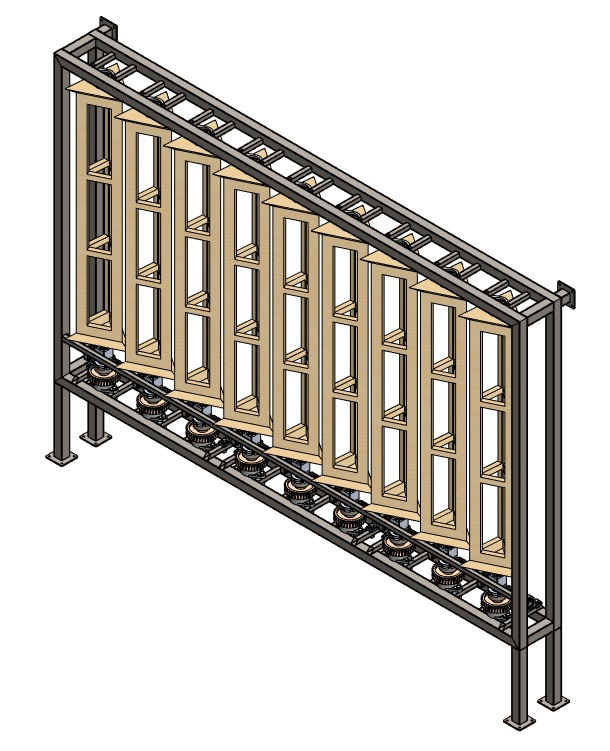
\includegraphics[width=1\textwidth]{imagenes/ConceptoSolucion.jpg}
    \caption{\footnotesize Concepto solución elegido}
    \label{fig:ConceptoSolucionElegido}
\end{figure}
\FloatBarrier
%------------------------------Elegido----------------------------------


%Imágenes del prototipo
